\documentclass[useAMS,usenatbib]{mn2e}
\usepackage{epsfig,rotate,graphicx}
\usepackage[fleqn]{amsmath}
\usepackage{subfigure}
\usepackage{lscape}
\usepackage{bm}
\usepackage{paralist}

\newcommand{\p}{\partial}
\newcommand{\mnras}{MNRAS}
\newcommand{\apj}{ApJ}
\newcommand{\na}{New A}
\newcommand{\aap}{A\&A}
\newcommand{\apjl}{ApJL}
\newcommand{\araa}{ARAA}
\newcommand{\dd}{\delta}
\newcommand{\adot}{\dot{a}}
\newcommand{\be}{\begin{equation}}
\newcommand{\ee}{\end{equation}}
\newcommand{\gtrsim}{\;\raisebox{-.8ex}{$\buildrel{\textstyle>}\over\sim$}\;}
\newcommand{\lesssim}{\; \raisebox{-.8ex}{$\buildrel{\textstyle<}\over\sim$}\;}
\newcommand{\anrev}{{\it ARA\&A, }}
\newcommand{\apjs}{{\it ApJS, }}
\newcommand{\icar}{{\it Icarus, }}
\newcommand{\mnr}{{\it MNRAS, }}
\newcommand{\nat}{{\it Nature, }}
\newcommand{\sci}{{\it Sci, }}
\newcommand{\ana}{{\it A\&A, }}
\newcommand{\anas}{{\it A\&AS, }}
\newcommand{\aaps}{{\it A\&AS, }}
\newcommand{\anar}{{\it A\&AR, }}
\newcommand{\prd}{{\it Phys. Rev. D }}
\newcommand{\qjl}{{\it QJRAS, }}
\newcommand{\sbar}{\bar{\sigma}}
\newcommand{\avg}[1]{\langle #1 \rangle}
%% \newcommand{\max}{\mathrm{max}}
%% \newcommand{\min}{\mathrm{min}}
\newcommand{\aziavg}[1]{\langle #1 \rangle_\phi}
\newcommand{\init}[1]{#1^{(0)}}
\newcommand{\bu}{\bm{u}}
\newcommand{\bv}{\bm{v}}
\newcommand{\rin}{r_\mathrm{in}}
\newcommand{\rout}{r_\mathrm{out}}
\newcommand{\dampin}{r_\mathrm{d,in}}
\newcommand{\dampout}{r_\mathrm{d,out}}
\newcommand{\psid}{\psi_\mathrm{d}}
\newcommand{\psitr}{\psi_\mathrm{tr}}
\newcommand{\psimax}{\psi_\mathrm{max}}
\newcommand{\Rtr}{R_\mathrm{tr}}
\newcommand{\lmax}{l_\mathrm{max}}
\newcommand{\mmax}{m_\mathrm{max}}
\newcommand{\trel}{t_\mathrm{rel}}
\newcommand{\zeus}{{\tt ZEUS-MP }}
\newcommand{\pluto}{{\tt PLUTO }}
\newcommand{\ii}{\mathrm{i}}
%\newcommand{\avg}[1]{\langle{#1}\rangle}
\DeclareMathOperator{\erf}{erf}




\title[Vortices in viscous discs]{Testing large-scale 
  vortex formation against viscous layers in three-dimensional discs}

%% \author[Lin]{ Min-Kai Lin
%%   \thanks{E-mail: mklin924@cita.utoronto.ca} \\ 
%% Canadian Institute for Theoretical Astrophysics,  
%% 60 St. George Street, Toronto, ON, M5S 3H8, Canada \\
%% }

\author[Lin and Umurhan]{ Min-Kai Lin$^1$
  \thanks{E-mail: mklin924@cita.utoronto.ca} and Orkan M. Umurhan $^2$ \thanks{E-mail:TBC} \\
  $^1$ Canadian Institute for Theoretical Astrophysics,
  60 St. George Street, Toronto, ON, M5S 3H8, Canada \\
  $^2$ TBC
}

\begin{document}

\maketitle
\begin{abstract}
  Vortex formation through the so-called Rossby wave 
  instability (RWI) in protoplanetary discs has been invoked to play a
  role in planet formation theory, and has been suggested to explain
  the observation of large dust asymmetries in transitional discs.   
  However, whether or not vortex-formation operates in layered
  accretion discs, i.e. models of protoplanetary discs including dead zones, 
  has not been verified. As a first step to test the robustness of
  vortex-formation through the RWI in 3D discs, we present customized
  non-linear hydrodynamical
  simulations of 3D protoplanetary discs with an imposed kinematic
  viscosity that is height-dependent. Two types of numerical 
  experiments are performed:
  \begin{inparaenum}[(i)]
  \item non-axisymmetric instability of artificial
    density bumps;  
  \item vortex-formation at planetary gap edges.%; and 
%  \item vortex-formation in discs with a radial viscosity transition.
  \end{inparaenum}
   We find, from the first experiment, that the linear instability is largely unaffected by viscosity and remains dynamical. 
  However this is assuming that a steady-state viscous disc with a density bump can be constructed.  The disc-planet simulations 
  also show the initial development of vortices at gap edges, but in layered discs the vortex is transient and disappears 
  well into the non-linear regime. Our experimental results suggest that vortex
  formation via the RWI may require low viscosity throughout the 
  vertical extent of the disc. 
\end{abstract}

\begin{keywords}
planetary systems: formation --- planetary systems:
protoplanetary discs
\end{keywords}


\section{Introduction}\label{intro}

%\begin{itemize}
%\item transitional disk observations. ALMA. large-scale
%  structures. %planet interpretation 
%\item planet(estimal) formation %alread invoked in planetestimal
%                                %formation (barge sommeria 95)
%\end{itemize}

Recent observations have revealed a class of transition discs ---
circumstellar discs which are dust poor in its inner regions ---  
with non-axisymmetric dust distributions in the outer disc
regions. One %some observations 
interpretation of such a non-axisymmetric structure is the presence of
a large-scale disc vortex, which is known to act as a dust trap
\citep{barge95}. Because of its occurence adjacent to the inner dust
hole, it has been suggested that such a vortex is a result of the
so-called Rossby wave instability: a hydrodynamical instability
associated with localized radial structures in thin discs.  

%2D results and relation to PPI
%linear stability analysis
%nonlinear simulations
%dust capture 

Modern studies of the RWI began with 2D linear stability analysis
\citep{lovelace99,li00}, which showed that a disc with localized
structure, such as a surface density enhancement over a
charactertistic lengthscale of the local scale-height, is unstable to
non-axisymmetric perturbations which grow on dynamical (orbital)
timescales. Early nonlinear 


%3D results
An important extension to the studies mentioned above is the
generalization of the RWI to 3D 
discs. Both nonlinear 3D hydrodynamic simulations 
\citep{meheut10,meheut12b,lin12b} and 3D linear calculations
\citep{umurhan10,meheut12,lin12,lin13} have been carried out. 
These studies reveal that the RWI is a 2D instability,
in that there is negligible difference between growth rates obtained
from 2D and 3D linear calculations. The associated density and
horizontal velocity perturbations have weak vertical dependence; and
vertical velocities are small. In nonlinear hydrodynamic simulations,
the vortices are columnar and extend throughout the vertical domain. 

%relevance to layered disc models
The RWI therefore appears to be a global instability in the direction
perpendicular to the disc midplane. Thus conditions away
from the disc midplane may have important effects on vortex-formation
via the RWI. For example, \cite{lin13a} only found linear
instability for certain upper disc boundary conditions. This issue is
relevant to protoplanetary disc models including `dead zones'. 

%the question
In layered protoplanetary disc models, accretion due to MRI turbulence
is small near the midplane (the dead zone), while MRI turbulence driven accretion
operaties near the disc surface \citep{gammie96,armitage11}. %also flemming, oishi, and the japanese guys  
If MRI-driven accretion can be modelled through an effective 
viscosity, this corresponds to a low-viscosity midplane and 
high-viscosity atmosphere. It is therefore valid to ask how such a
vertical disc structure would affect the RWI. 

This issue is partly motivated by viscous disc-planet
simulations show that the RWI only develops when the viscosity is
sufficiently small \citep{valborro07}%and edgar 'vertical structure of gaps'
A natural question one may pose is this: what if the effective 
viscosity near the midplane is sufficiently low for the RWI to
develop, but is too high away from the midplane? Does the
instability, and therefore vortex-formation, still take place? 

In this work we examine vortex formation through the RWI in
layered discs. As a first study to this problem, we take an
experimental approach through customized numerical hydrodynamic
simulations. We simulate 3D protoplanetary discs with an imposed
kinematic viscosity that varies with height above the disc
midplane. %because most simulations use a NS viscosity. full mri
          %simulation too expensive. comparison to previous 


%Apart from simplicitly, hydrodynamic models also allow 
%computations to be completed with reasonable cost. It is, however,
%still questionable as to whether or not an explicit viscosity 

%what we're going to do
%expensive 3D calcs. can't do parameter survey
%example sim demonstrating effect of layered disc
%highlight the potential importance of disc vertical structure
%need to know it can operate in typical disc conditions before
%invoking it to explain observations

%our approach to this problem will be through customized viscous disc
%simulations. we therefore utilize toy models in which we have full
%control. 




\section{Disc model and Governing equations}\label{model} 
We consider a three-dimensional, {\bf locally} isothermal,
non-self-gravitating fluid disc orbiting a central 
star of mass $M_*$. {\bf We adopt a non-rotating frame centred on the
  star. Our computer simulations employ spherical co-ordinates
  $\bm{r}=(r,\theta,\phi)$, but for model description and results 
  analysis we will also use cylindrical co-ordinates $\bm{r}=(R, \phi,
  z)$.} We also define $\psi \equiv \pi/2 -
\theta$ as the angular displacement from the disc midplane. For
convenience, we will sometimes refer to $\psi$ as the vertical
direction. The governing equations are: 
\begin{align}
  &\frac{\p\rho}{\p t} + \nabla\cdot\left(\rho\bm{v}\right) =
  0,\label{cont_eq}\\ 
  &\frac{\p\bm{v}}{\p t} + \bm{v}\cdot\nabla\bv = -\frac{1}{\rho}\nabla
  p -\nabla{\left(\Phi_*+\Phi_p\right)} +\bm{f}_\nu + \bm{f}_d\label{mom_eq},    
\end{align}
where $\rho$ is the mass density, $\bv$ is the velocity field (the
azimuthal angular velocity being $\Omega\equiv v_\phi/R$) and 
$p=c_s^2\rho$ is the pressure. 
The sound speed $c_s$ is prescribed as 
\begin{align}
  c_s = hr_0\Omega_k(r_0)\times\left(\frac{r_0}{R}\right)^{q/2}, 
\end{align}
where $h$ is the aspect-ratio at the reference radius $r_0$, 
$\Omega_k(R) = \sqrt{GM_*/R^3}$ is the Keplerian frequency and $G$ is
the gravitational constant. The power-law index $q$ specifies the
radial temperature profile: $q=0$ corresponds to a strictly isothermal
disc, while $q=1$ is a locally isothermal disc with constant aspect
ratio. In Eq. \ref{mom_eq}, $\Phi_*(r) = -GM_*/r $ is the stellar
potential and $\Phi_p$ is a planetary potential (see \S\ref{planet}
for details).  

Two dissipative terms are included in the momentum, equations: viscous
damping $\bm{f}_\nu$ and frictional damping $\bm{f}_d$. The viscous
force is 
\begin{align}
  \bm{f}_\nu = \frac{1}{\rho}\nabla\cdot\bm{T},
\end{align}
where 
\begin{align}
  \bm{T} = \rho\nu \left[\nabla\bv + \left(\nabla\bv\right)^\dagger
    - \frac{2}{3}\left(\nabla\cdot\bv\right)\bm{1} \right]
\end{align}
is the viscous stress tensor and $\nu$ is the kinematic viscosity 
($^\dagger$ denotes the transpose). The frictional force is 
\begin{align}
  \bm{f}_d = -\gamma\left(\bv - \bv_\mathrm{ref}\right),
\end{align}
where $\gamma$ is the damping coefficient and
$\bm{v}_\mathrm{ref}$ is a reference velocity field. 
$\nu$ and $\gamma$ are prescribed functions of position only (see
below). %The kinematic viscosity $\nu$ is specified directly, but
%conversion to an alpha parameter 

\subsection{Disc model and initial conditions}\label{IC}
The numerical disc model occupies $r\in[\rin,\rout]$,
$\theta\in[\theta_\mathrm{min}, 
  \pi/2]$ and $\phi\in[0,2\pi]$ in spherical co-ordinates. 
Only the upper disc is simulated explicitly 
($\psi>0$), by assuming symmetry across the midplane. The maximum
angular height is $\psimax \equiv \pi/2 - \theta_\mathrm{min}$. 
The extent of the vertical domain is parametrized by $n_h\equiv
\tan{\psimax}/h$, i.e. the number of scale-heights at the reference 
radius.   

The disc is initially axisymmetric with zero cylindrical vertical
velocity: $\rho(t=0)\equiv\rho_i(R,z)$ and
$\bm{v}(t=0)\equiv(v_{Ri}\,, R\Omega_i\,, 0)$ in cylindrical
co-ordinates. The initial density field is set by assuming vertical
hydrostatic balance between gas pressure and stellar gravity:
\begin{align}\label{vert_balance}
  0 = \frac{1}{\rho_i}\frac{\p p_i}{\p z} + \frac{\p \Phi_*}{\p z},
\end{align}
where $p_i=c_s^2\rho_i$ is the initial pressure field. We write 
\begin{align}\label{init_den}
  \rho_i = \frac{\Sigma_i(R)}{\sqrt{2\pi}H(R)}
  \exp{\left\{\frac{1}{c_s^2}\left[\Phi_*(R) - \Phi_*(r)\right]\right\}},
\end{align}
where $H = c_s/\Omega_k$ is the pressure scale-height. The initial
surface density $\Sigma_i(R)$ is chosen as  
\begin{align}
  \Sigma_i(R) = \Sigma_0\left(\frac{R}{r_0}\right)^{-\sigma}\times B(R),
  %\left(1 - \sqrt{\frac{R_\mathrm{in}}{R + H_\mathrm{in}}}\right)\times B(R),
\end{align}
where $\sigma$ is the power-law index, and the surface density scale $\Sigma_0$ 
is arbitrary for a non-self-gravitating disc. 
The bump function $B(R)$ is 
\begin{align}\label{bump_func}
B(R) = 1 + \left(A - 1\right)\exp{\left[-\frac{(R-r_0)^2}{2\Delta R^2}\right]},
\end{align}
where $A$ is the bump amplitude and $\Delta R$ is the bump width. The
initial surface  
density has bump if $A>1$ and is smooth if $A=1$. 

The initial angular velocity is chosen to 
satisfy centrifugal balance with pressure and stellar gravity: 
\begin{align}\label{init_vphi} 
  R\Omega^2_i = \frac{1}{\rho_i}\frac{\p p_i}{\p
    R} + \frac{\p\Phi_*}{\p R},  
\end{align}
so $\Omega_i=\Omega_i(R)$ for a strictly isothermal equation of
state ($q=0$). 
%% Note that Eq. \ref{init_den} and Eq. \ref{init_vphi} are the
%% vertical and cylindrical radial momentum equations assuming a steady
%% state and negligible viscosity. 

The initial cylindrical radial velocity $v_{Ri}$ and the viscosity
profile $\nu$ depends on the numerical experiment, and will be
described along with simulation results. Note that $v_{Ri}$ and $\nu$
are not independent if one additionally requires a steady-state (see
\S\ref{density_bump}).    

\subsection{Damping}
We apply frictional damping in the radial direction to reduce
reflections from boundaries \citep[e.g.][]{bate02,valborro07}.  The
damping coefficient $\gamma$ is only  non-zero within the `damping
zones', here taken to be $r\leq \dampin,\,  
r\geq \dampout$, 
\begin{align}
  \gamma = \hat{\gamma}\Omega_i\times
  \begin{cases}
    \xi_\mathrm{in}(r) & r\leq\dampin \\
    \xi_\mathrm{out}(r) & r\geq\dampout \\
  \end{cases},
\end{align}
where $\hat{\gamma}$ is the dimensionless damping rate. We choose
\begin{align}
  \xi_\mathrm{in}(r) = \left(\frac{\dampin - r}{\dampin - \rin}\right)^2 \text{ and } \quad
  \xi_\mathrm{out}(r) = \left(\frac{r - \dampout}{\rout- \dampout}\right)^2
\end{align}
for the inner and outer radial zones, respectively. 

\subsection{Planet potential}\label{planet}
Our disc model has the option to include a planet potential $\Phi_p$,
\begin{align}
  \Phi_p(\bm{r},t) = -\frac{GM_p}{\sqrt{|\bm{r}-\bm{r}_p(t)|^2 +
      \epsilon^2_p}} + \frac{GM_p}{|\bm{r}_p|^3}\bm{r}\cdot\bm{r}_p,
\end{align}
where $M_p$ is the planet mass,
$\bm{r}_p(t)~=~(r_0,\,\pi/2,\,\Omega_k(r_0)t+\pi)$ its position in
spherical co-ordinates, $\epsilon_p = \epsilon_{p0}r_h$ is a
softening length, and $r_h=(M_p/3M_*)^{1/3}r_0$ is the Hill radius. 
For the purpose of our study $\Phi_p$ is considered as a 
fixed external potential. That is, orbital migration is neglected. 

\section{Numerical experiments}\label{sims}
The neccessary condition for the RWI --- a potential vorticity 
extremum --- is either set as an initial condition via a density bump, 
or obtained from a smooth disc by evolving it under disc-planet
interaction. The setup of each experiment is detailed in subsequent
sections.    

We adopt units such that $G=M_*=1$, and the reference radius $r_0=1$.    
We set $\sigma=0.5$ for the initial surface density profile and apply 
frictional damping within the shells $r<r_\mathrm{d,in} = 1.25\rin$
and $r>r_\mathrm{d,out}=0.84\rout$.

The fluid equations are evolved using the \pluto code \citep{mignone07} with 
the FARGO algorithm enabled\citep{mignone12}. We employ a static
spherical grid with $(N_r, N_\theta, N_\phi)$ zones uniformly spaced
in all directions. For the present simulations the code was configured
with piece-wise linear reconstruction, a Roe solver and second order
Runge-Kutta time integration.   

Boundary conditions are imposed through ghost zones.   
Let the flow velocity parallel and normal to a boundary be
$v_\parallel$ and $v_\perp$, respectively. %($v_\perp>0$ signifies flow
%out of the computational domain.) 
Two types of numerical 
conditions are considered for the meridional boundaries:
\begin{inparaenum}[(a)]
\item \emph{reflective}: $\rho$ and $v_\parallel$ are symmetric with
  respect to the boundary while $v_\perp$ is anti-symmetric;  
  %% \item \emph{outflow}, ghost values of $\rho,\,v_\parallel$ set to that of the nearest active zone, 
  %% likewise for $v_\perp$ but only if the active $v_\perp>0$, otherwise ghost values of $v_\perp$ are set to zero; 
\item \emph{unperturbed}: ghost zones retain their initial values
\end{inparaenum}.
The boundary conditions adopted for all simulations is unperturbed in
$r$, reflective in $\theta$ and periodic in $\phi$. 

%For all cases both radial boundaries are unperturbed and the midplane is reflective. 

\subsection{Diagnostics}
We list several quantities calculated from simulation data for use in
result visualization and analysis.  
%Averaged quantities are used to facilitate  
%comparison between different cases. We use $\avg{\cdots}_j$ 
%to denote spatial averaging along the $j^\mathrm{th}$ co-ordinate. 
%Azimuthal averages are taken over $\phi\in[0,2\pi]$, while the domain
%for meridional averaging is stated along with simulation results in
%the next section. %% We also use $\overline{\cdots}$ to denote a further
%% time average. 

\subsubsection{Density perturbations}
The relative density perturbation $\delta\rho$ and 
and the non-axisymmetric density fluctuation are defined as 
\begin{align}
  \delta\rho(\bm{r},t) \equiv \frac{\rho - \rho_i}{\rho_i}, \quad
  \Delta\rho(\bm{r},t) \equiv \frac{\rho -
    \aziavg{\rho}}{\aziavg{\rho}}, 
\end{align} 
where $\avg{\cdot}_\phi$ denotes an azimuthal average.  
Note that in general $\Delta\rho$ accounts for the time evolution of
the axisymmetric part of the density field, but if
$\p_t\avg{\rho}_\phi=0$ then $\Delta\rho$ is identical to
$\delta\rho-\avg{\delta\rho}_\phi$.   

\subsubsection{Vortical structures}
The Rossby number
\begin{align}
  Ro \equiv
  \frac{\hat{\bm{z}}\cdot\nabla\times\bv-\avg{\hat{\bm{z}}\cdot\nabla\times\bv}_\phi}{2\aziavg{\Omega}},   
\end{align} 
can be used to quantify the strength of vortical structures and to
visualize it. $Ro<0$ signifies anti-cyclonic motion with respect to
the axisymmetric shear. Note that while for thin discs the rotation
profile is Keplerian, the shear is non-Keplerian for radially  
structured discs (i.e. $\Omega\simeq\Omega_K$ but
$\kappa\neq\Omega$). 

\subsubsection{Potential vorticity}
The potential vorticity (PV, or vortensity) is defined as
%\begin{align}
$  \bm{\eta}_\mathrm{3D} = \nabla\times\bm{v}/\rho. $
%\end{align}
%% Accordingly we defined the density-weighted average
%% \begin{align}
%%   \bm{\eta} = \frac{\int \rho\bm{\eta}_\mathrm{3D} dz}{\int\rho dz}. 
%% \end{align}
%% We are usually interested in the $z$-component of the PV, 
Since we are considering geometrically thin discs, however, it will be
convenient to work with vertically averaged quantities. Specifically,
we define 
\begin{align}
  \eta_z = \frac{1}{\Sigma}\int \hat{\bm{z}}\cdot\nabla\times\bv dz
\end{align}
as the PV in this paper, where $\Sigma = \int\rho dz$ and the
integrals are confined to the computational domain. 

We recall for a two-dimensional disc the vortensity is defined as 
$\eta_\mathrm{2D} \equiv \hat{\bm{z}}\cdot\nabla\times\bv/\Sigma$, and
extrema in $\eta_\mathrm{2D}$ is neccessary for the RWI in
2D \citep{lovelace99,lin10}. Clearly, if the velocity field has no
vertical dependence then $\eta_z$ is proportional to
$\eta_\mathrm{2D}$ (at fixed cylindrical radius).   

\subsubsection{Perturbed kinetic energy density}  
We will be interested in the energetics of non-axisymmetric
structures. We define the perturbed kinetic energy as
$W\equiv|\bm{v}|^2/|\bm{v}(t~=0)|^2 - 1$, and its Fourier transform 
$W_m\equiv\int_0^{2\phi} W\exp{(-\mathrm{i}m\phi)}d\phi$. We will examine
$|W_m(r,\theta)|$ averaged over portions of the $(r,\theta)$
plane. %Specifically we define the `midplane energy' as $|W_m|$
%averaged over $$

\section{Non-axisymmmetric instability of artificial density bumps in
  layered discs}\label{density_bump} 
We first consider discs initialised with a density bump. Our aim here
is to examine the effect of (layered) viscosity on the RWI 
\emph{through the linear perturbation}. 
In general a density bump in a viscous disc will undergo viscous
spreading \citep{lyndenbell74}, but it is possible to 
avoid this by choosing a viscosity profile $\nu$ and initial cylindrical radial
velocity $v_{Ri}$ appropriately. 
Although artificial, this setup avoids 
the simultaneous evolution of the density bump subject to
axisymmetric viscous spreading and growth of
non-axisymmetric perturbations; the latter of which is our focus. 


\subsection{Viscous equilibria for a radially structured
  disc}\label{visc_eq} 
%The RWI is a linear instability. That is, non-axisymmetric 
%disturbances grow exponentially with respect to a time-independent
%axisymmetric background. A convenient way to study the RWI is to
%initialize an inviscid disc with a density bump \citep[e.g.][]{li00}. 
%However, taking this approach with a viscous disc is problematic,
%because the density bump will generally undergoe viscous spreading 
%\citep{lyndenbell74}. 
 
In choosing $\rho_i$ and $\Omega_i$, we neglected radial
velocities and viscous forces in the steady-state vertical and
cylindrical radial momentum equations (Eq. \ref{vert_balance} and
Eq. \ref{init_vphi}, respectively). This is standard practice for
accretion disc modelling \citep[e.g.][]{takeuchi02}.   

However, $v_{R}$ and $\nu$ cannot be ignored in the azimuthal
momentum equation. Indeed, if a steady-state is desired, then the
conservation of angular momentum in a viscous disc implies special
relations between the viscosity, cylindrical radial velocity and
density field. %We do this for simulations in \S\ref{density_bump}.   


\subsubsection{Initial cylindrical radial velocity}
For axisymmetric flow with angular velocity that only depends on the
cylindrical radius, the azimuthal momentum equation reads 
\begin{align}\label{ang_mom_cons}
  R\rho v_R\frac{\p}{\p R}\left(R^2\Omega \right) = \frac{\p}{\p
    R}\left(R^3\rho\nu\frac{\p\Omega}{\p R}\right). 
\end{align}
Assuming a steady state with $v_z=0$, mass
conservation (Eq. \ref{cont_eq}) implies that the mass flux  
$\dot{M}\equiv R\rho v_R$ is independent of $R$. In this case,
Eq. \ref{ang_mom_cons} can 
be integrated once to yield 
\begin{align}\label{temp}
  \dot{M}R^2\Omega = R^3\rho\nu\Omega^\prime + C(z) \quad \text{if $\p_R\dot{M}$} = 0, 
\end{align}
where $^\prime$ denotes $d/dR$ and $C(z)$ is an arbitrary function of
$z$. Eq. \ref{temp} motivates the simple choice
\begin{align}\label{init_vr} 
  v_{Ri} = \frac{\nu}{R}\frac{d\ln{\Omega_i}}{d\ln{R}} 
\end{align}
for the initial cylindrical radial velocity. Next, we choose the
viscosity profile $\nu$ to make the mass flux independent of
cylindrical radius.  

\subsubsection{Viscosity profile for a steady state}\label{visc_model}
If the initial conditions corresponds to a steady state, then
$R \rho_i v_{Ri}$ can only be a function of $z$. With $v_{Ri}$ chosen
by Eq. \ref{init_vr}, this implies 
$R\rho_i\nu\Omega_i^\prime/\Omega_i$ is only a function of $z$. We are
therefore free to choose the vertical dependence of viscosity.   

Let $\nu = \hat{\nu}r_0^2\Omega_K(r_0)$, where
$\hat{\nu}=\hat{\nu}(R,z)$ is a dimensionless function describing
the magnitude and spatial distribution of the axisymmetric kinetmatic
viscosity. We choose $\hat{\nu}$ such that   
\begin{align}\label{visc_profile}
  \hat{\nu}\rho_i(R,z)\frac{d\ln{\Omega_i}}{d\ln{R}} =
  \hat{\nu}_0\left[1+Q(z/H_0)\right]\rho_i(r_0,z)\left.\frac{d\ln{\Omega_i}}{d\ln{R}}\right|_{r_0}, 
\end{align}
where $\nu_0$ is a constant dimensionless floor viscosity and   
\begin{align}\label{step}
  Q(\zeta) = \frac{\left(A_\nu - 1\right)}{2}
  \left[  2 + \tanh{\left(\frac{\zeta - \zeta_\nu}{\Delta\zeta_\nu}\right)}
    %  \left. 
    - \tanh{\left(\frac{\zeta +
        \zeta_\nu}{\Delta\zeta_\nu}\right)}\right]
\end{align}
is a generic function describing a step of magnitude
$A_\nu-1$. The position and width of the step is described by
$\zeta_\nu$ and $\Delta\zeta_\nu$, respectively. 
In Eq. \ref{visc_profile} we have set the dimensionless co-ordinate
$\zeta=z/H_0$ where $H_0=H(r_0)$. We have specified
the kinematic viscosity directly, but it is straight forward to
translate $\hat{\nu}$ to an alpha viscosity 
using $\nu = \alpha c_s H$ \citep{shakura73}. This gives $\alpha =
\hat{\nu}/h^2$ at $R=r_0$.  Thus for $h=0.1$ and $\hat{\nu}=10^{-4}$ we
get $\alpha\sim 10^{-2}$.  

Eq. \ref{visc_profile} implies that at the fixed cylindrical radius
$R=r_0$, the dimensionless viscosity increases from $\hat{\nu} =
\hat{\nu}_0$ at the midplane to $\hat{\nu} = A_\nu\hat{\nu}_0$ for
$z > \zeta_\nu H_0$. An example of such a layered viscosity profile
profile is depicted in Fig. \ref{visc2d}. 
 

\begin{figure}
  \centering
  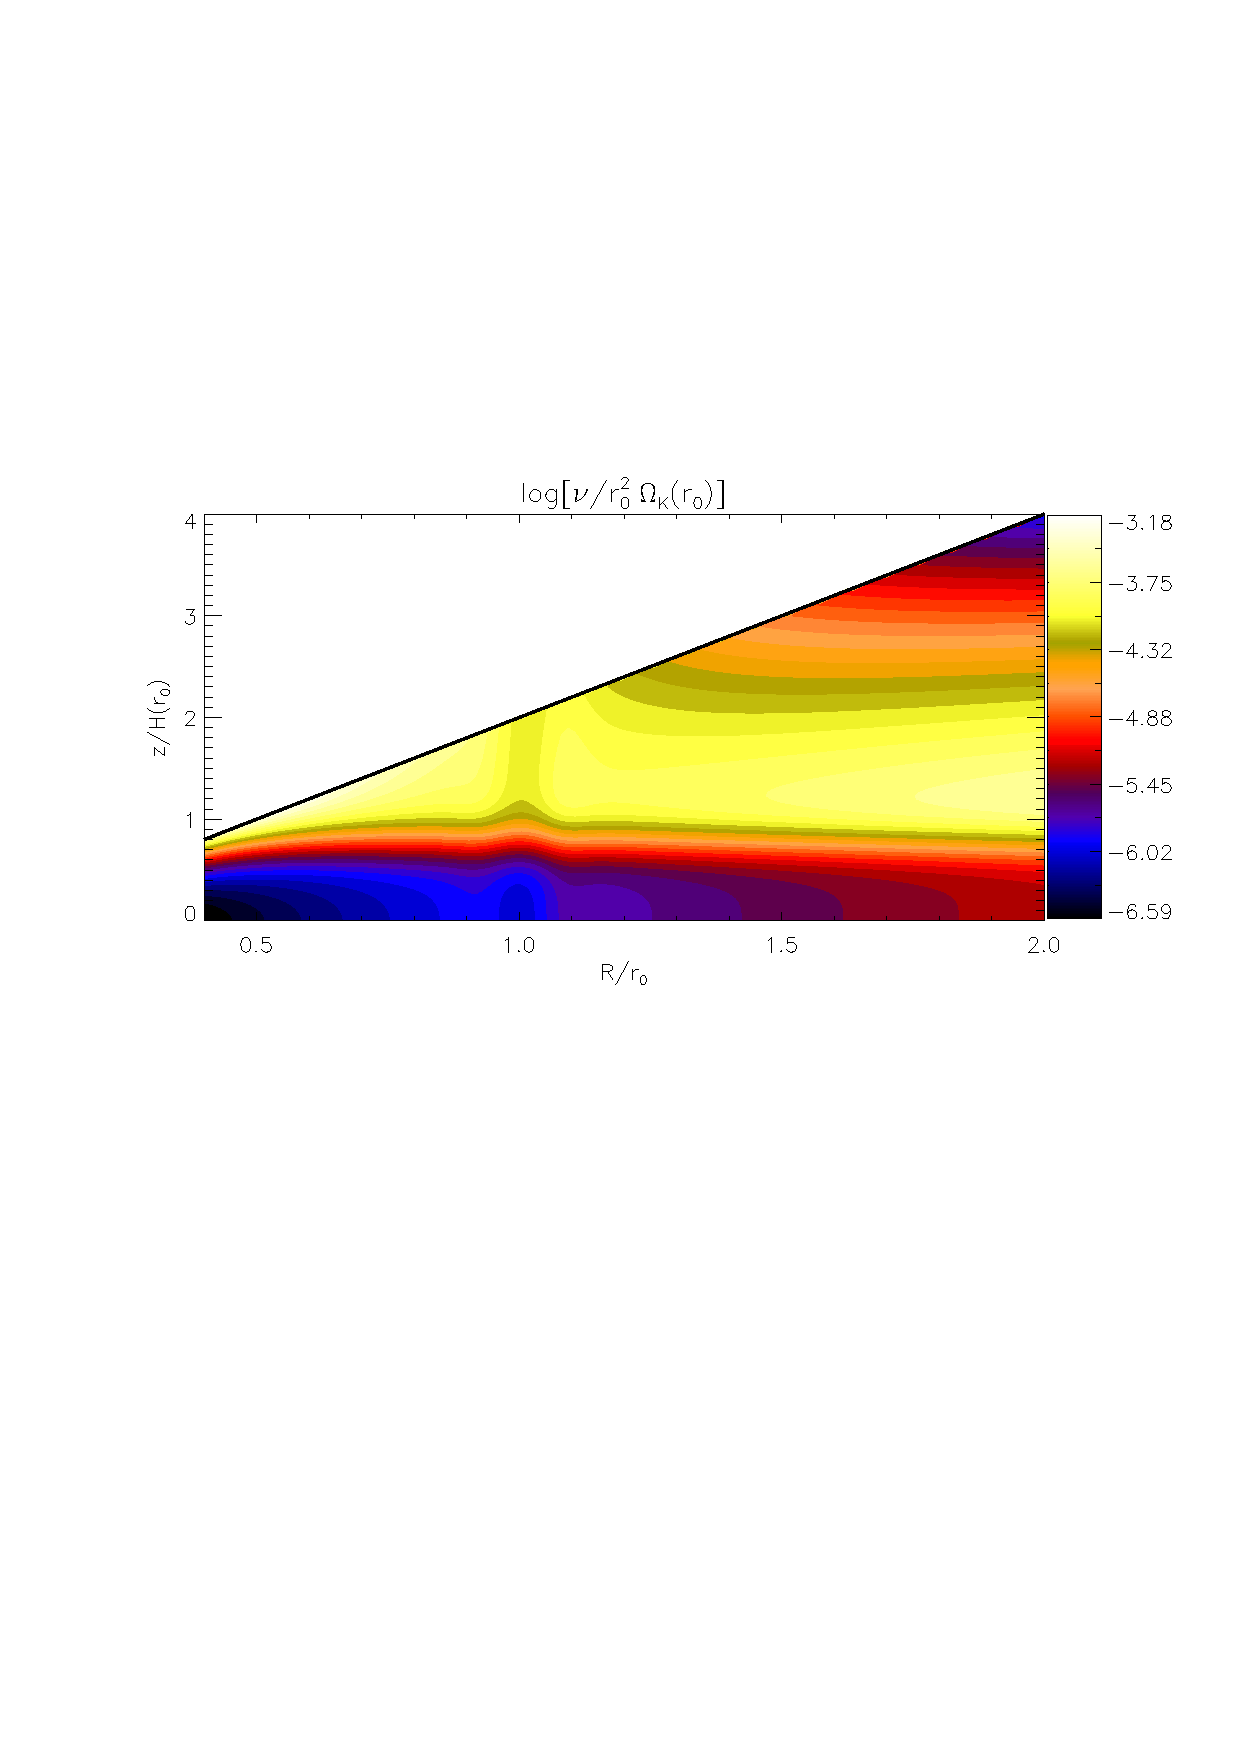
\includegraphics[width=\linewidth]{figures/pdisk_visc2d_layer2}
  \caption{Example of a two-layered kinematic viscosity profile
    resulting from Eq. \ref{visc_profile}. This specific plot
    corresponds to case V2. The solid line
    delineates the upper boundary of the computational domain.
    \label{visc2d}}
\end{figure}



\subsection{Simulations}
We consider discs with radial extent $[\rin,\rout]=[0.4,2.0]r_0$,
vertical extent with $n_h=2$ scale-heights and aspect-ratio $h=0.1$ at
$R=r_0$. We use $(N_r, N_\theta,
N_\phi)=(256,64,512)$ grid points. 
The resolution at the reference radius is then
$16,\,32,\,8$ cells per scale-height in $r,\theta,\phi$ directions,
respectively. The planetary potential is disabled for these runs
($M_p\equiv 0$).    

The bump parameters are set to $A=1.25$ and $\Delta R = 0.05r_0$ for
all runs in this section. The spherical radial velocity is subject 
to random perturbations of magnitude $10^{-4}c_s$ 
a few time-steps after initialisation. 

\subsubsection{Inviscid run}
For reference we simulate an effectively inviscid disc, case B0,
with the viscosity parameters $\hat{\nu}_0=10^{-9}$ and $A_\nu = 1$.  
The latter implies the viscosity is independent of $z$ at $R=r_0$.   
Inviscid setups similar to case B0 have previously been simulated
both in the linear and nonlinear regimes  \citep{meheut12, lin13}. So,
in addition to a control run, case B0 also serves to test the \pluto
code in simulating the RWI.    

\subsubsection{Viscous runs}
In these runs the floor viscosity is 
$\hat{\nu}_0=10^{-6}$. The control run case V0 has $A_\nu =
1$. Thus, case V0 is the viscous version of case B0.  
We then consider models where the kinematic viscosity increases by
a factor $A_\nu=100$ for $z>\zeta_\nu H_0$ at the bump radius. We
choose $\zeta_\nu=1.5,\,1.0$ for cases V1 and V2, respecively.  This gives a upper 
viscous layer of thickness $0.5H$ and $H$ at $R=r_0$. (See
Fig. \ref{visc2d} for a plot of the kinematic viscosity profile for case V2.) 
For case V1 and V2 the transition thickness is fixed to
$\Delta\zeta_\nu=0.2$.  
 
Finally, we consider a high viscosity run, case V3, with $\zeta_\nu =
0$, i.e. the viscous layer occupies the entire vertical domain. This
is equivalent to setting $\hat{\nu}_0=10^{-4}$ and $A_\nu=1$.  

\subsubsection{Linear growth rates and frequencies}
The present setup allows us to define a linear instability in the
usual way: exponential growth of perturbations measured with respect
to an axisymmetric steady equilibrium. Although a proper linear
stability analysis, including the full viscous stress tensor, is
beyond the scope of this paper, we can nevertheless extract linear 
mode growth rates from the early evolution of nonlinear simulations.  

%For quantitative analysis of non-axisymmetric density structures, 
The $m^\mathrm{th}$ Fourier component of the density field is  
\begin{align}
\hat{\rho}_m(r,\theta,t) \equiv \int_0^{2\pi} \rho(\bm{r},t)\exp{(-\ii m\phi)}d\phi.
\end{align}
The magnitude of a Fourier mode is measured by 
\begin{align} 
a_m(t)\equiv \frac{b_m(t)}{b_0(0)},\quad b_m(t)\equiv \avg{|\hat{\rho}_m|}_r,
\end{align} 
where $\avg{\cdot}_r$ denotes averaging over a spherical shell (to be
chosen later). 
The complex frequency $\sigma_m$ associated with the $m^\mathrm{th}$ component 
is defined through 
\begin{align}\label{sigma}
  \frac{\p\hat{\rho}_m}{\p t} \equiv -\ii\sigma_m\hat{\rho}_m. 
\end{align}
The time derivative in Eq. \ref{sigma} can be computed implicitly by 
Fourier-transforming the continuity equation \citep[as done
  in][]{lin13}. 

%Note that we have defined the complex frequency as one would in a
%linear stability analysis because the RWI is a linear 
%instability. %% This definition is useful in assessing how the linear is
%% affected by the various boundary effects in the
%% linear phase (i.e. when perturbations are small). 
%The mode frequency defined here is therefore most appropriate to
%describe simulations where the axisymmetric background does not evolve
%in time (i.e. if $\p_t\avg{\rho}_\phi=0$), as required to define a
%linear instability. 

In a linear stability problem $\sigma_m$ is a constant eigenvalue. 
However, when extracted numerically from a non-linear simulation, 
we will generally obtain $\sigma_m=\sigma_m(r,\theta,t)$. Thus, we compute 
$\avg{\sigma_m}_r = m\omega_m + \ii q_m$    
where $\omega_m$ is the mode frequency and $q_m$ is the growth rate.
We normalise the linear frequencies by
$\Omega_0\equiv\Omega_i(r_0)\simeq\Omega_K(r_0)$. 

\subsection{Results}
Table \ref{artificial_bump} summarises the simulations presented in
this section.%, along with several diagnostic measures 
%of each case.  
 The linear mode frequencies are measured at 
$t=10P_0$ and averaged over the shell $r\in[0.8,1.2]r_0$.   
For convenience we will refer to $t\leq10P_0$ as the `linear
phase' since the relative density perturbations are
small ($\delta\rho\ll 1$) during this time.  
%The dominant azimuthal wavenumber is the mode with largest
%amplitude. 
The second set of measurements is made at $t=100P_0$, which is well
into the nonlinear regime. %The dominant mode is that with 
%$\mathrm{max}[a_m(100P_0)]$. 
The minimum Rossby number is measured at the midplane. 

\begin{table*}
  \centering
  \caption{Summary of hydrodynamic simulations initialized with a
    density bump. %% `UBC' is
    %% the boundary condition applied at the upper disc boundary. 
    Note that case V3
    is equivalent to setting 
    $\hat{\nu}_0=10^{-4}$ and $A_\nu=1$. \label{artificial_bump}}
  \begin{tabular}{lcccccl @{\extracolsep{0.1cm}} ccc}
    \hline\hline
    \multicolumn{4}{c}{\phantom{stuff}} &
    \multicolumn{3}{c}{$t = 10P_0$ (linear phase)}&
    \multicolumn{3}{c}{$t=100P_0$}\\
    \cline{5-7}\cline{8-10}
    Case  & $\log{\hat{\nu}_0}$ & $A_\nu$ &$\zeta_\nu$ & $m$ &
    $\omega_m/\Omega_0$ &
    $q_m/\Omega_0$ &  
    $m$ & $10^2a_m$ & $\mathrm{min}[Ro(z=0)]$ \\ 
    \hline
    B0 &-9 & 1 &n/a & 4 & 0.985  & 0.199  %omit = 3
    &  1 & 8.5  & -0.15   \\  
    
    V0  &-6 & 1 &n/a &  4 & 0.985  & 0.199   
    & 1 & 6.8 &  -0.11  \\
    
    V1  &-6 & 100 & 1.5  & 4 & 0.986  & 0.191
    &  1 & 7.8 &  -0.19 \\
    
    V2  & -6 & 100 & 1.0  &  4  & 0.986  & 0.182  
    &  1 & 4.9 &  -0.21 \\
    
    V3  & -6 & 100 & 0.0  &  4  & 0.986  &  0.131  
    &  3 &  3.7  &  -0.25 \\
   \hline
  \end{tabular}
\end{table*}

\subsubsection{Inviscid reference case}
Fig. \ref{bump0_bump1} 
shows the density fluctuation and Rossby number for
case B0. The dominant linear mode is $m=4$ with a growth rate
$0.2\Omega_0$. This 
corresponds to a growth timescale of $\sim P_0$. 
This is consistent with recent 3D linear calculations
\citep{meheut12,lin13}. Fig. \ref{bump0_bump1} shows that the
linear phase consists of non-axisymmetric vorticity perturbations on
either side of the density bump \citep{umurhan10}, i.e. vorticity
waves propagating along the PV gradients.     

The nonlinear outcome of the RWI is vortex-formation
\citep{li00}. Four vortices develop initially, but 
merge on a dynamical time-scale to produce 
a single vortex. %meheut12 vortex weakens on even longer time scales
                 %but we do not consider it here 
 Case B0 evolves similarly to previous numerical  
studies of the RWI in an inviscid disc
\citep[e.g.][where more detailed analyses are 
given]{meheut10,meheut12b}. This, together with the agreement with
previous linear simulations, demonstrates the ability of the \pluto
code to capture the RWI. 

\begin{figure}
  \centering
  \includegraphics[scale=.27,clip=true,trim=0cm 0.9cm 0cm
    0cm]{figures/bump0_pdisk001}\includegraphics[scale=.27,clip=true,trim=2.3cm
    0.9cm 0cm
    0cm]{figures/bump0_pdisk005}\includegraphics[scale=.27,clip=true,clip=true,trim=2.3cm
    0.9cm 0cm
    0cm]{figures/bump0_pdisk010}
   \includegraphics[scale=.27,clip=true,trim=0cm 0.cm 0cm
     0.9cm]{figures/bump0_vort001}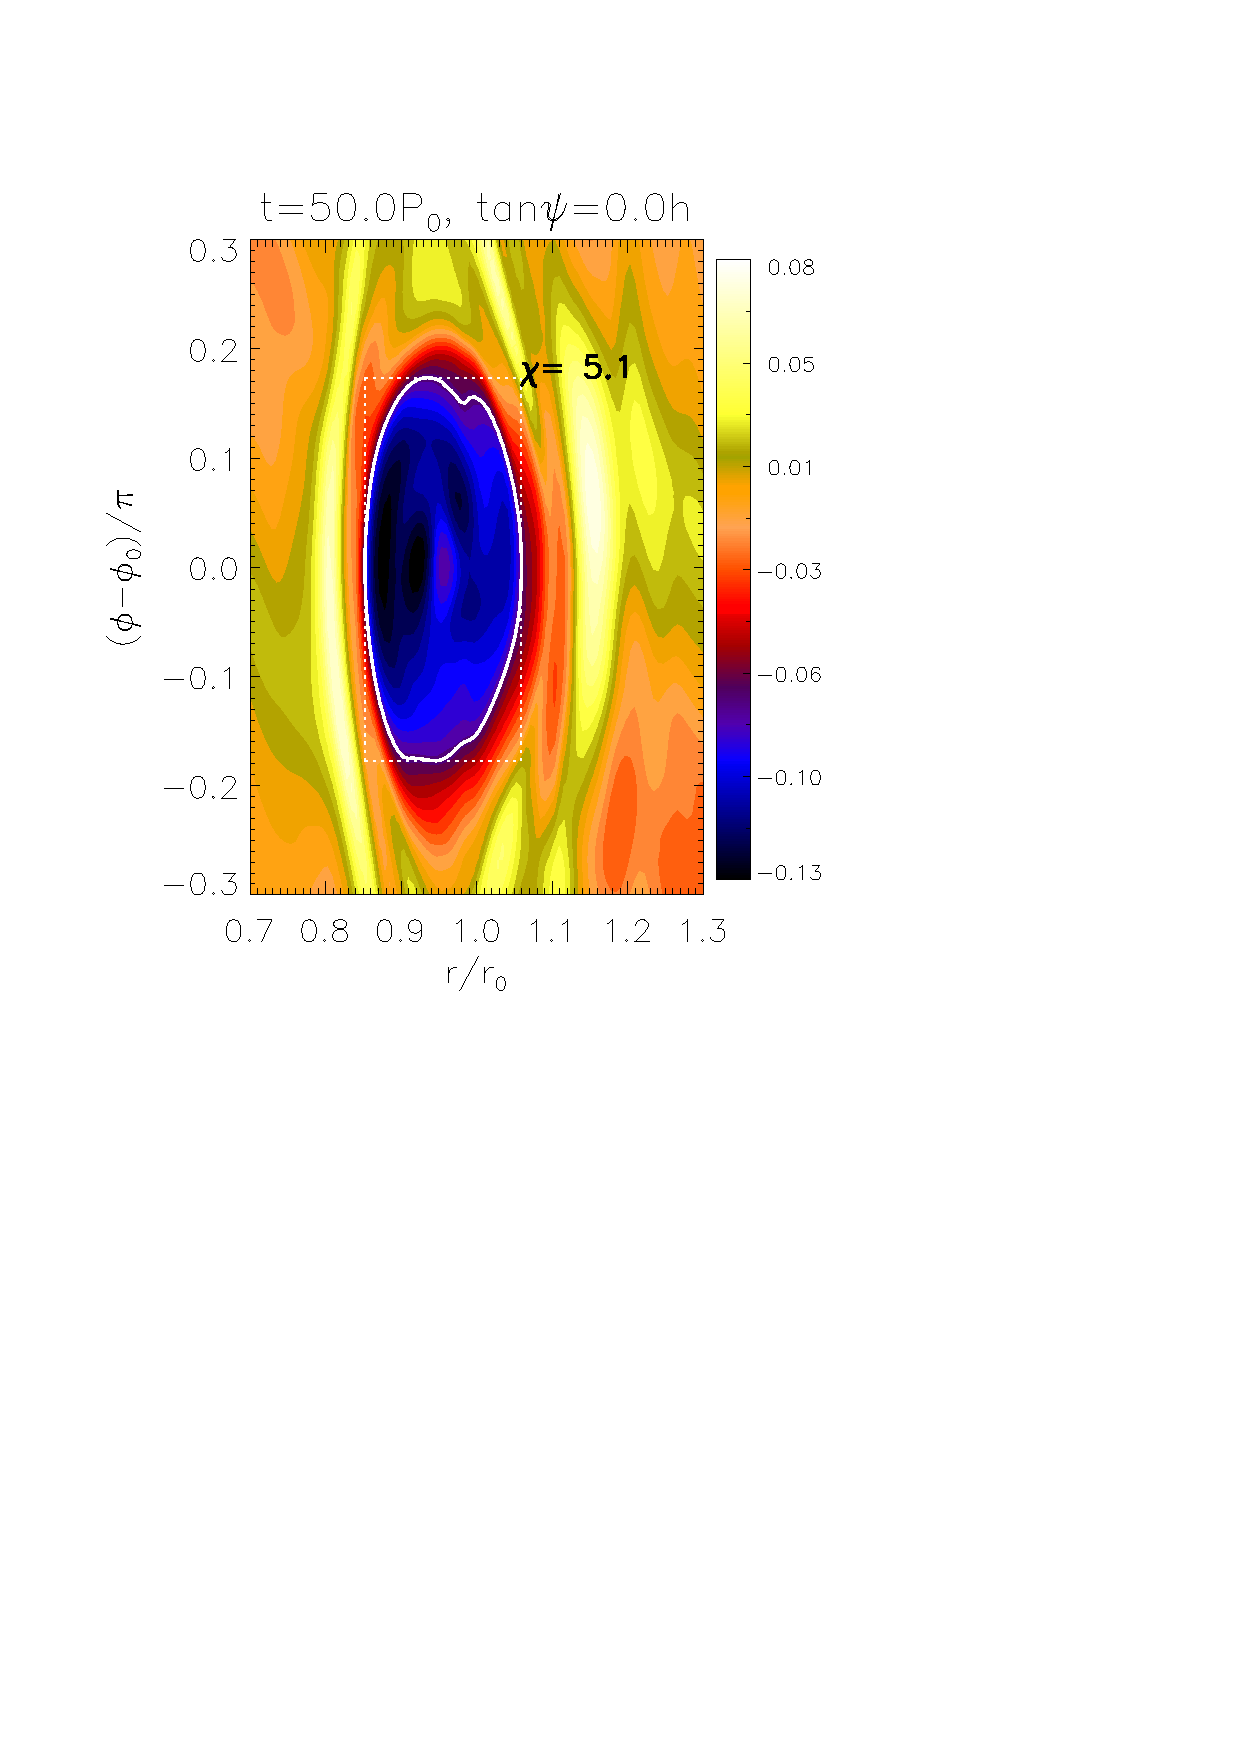
\includegraphics[scale=.27,clip=true,trim=2.3cm
     0.cm 0cm
     0.9cm]{figures/bump0_vort005}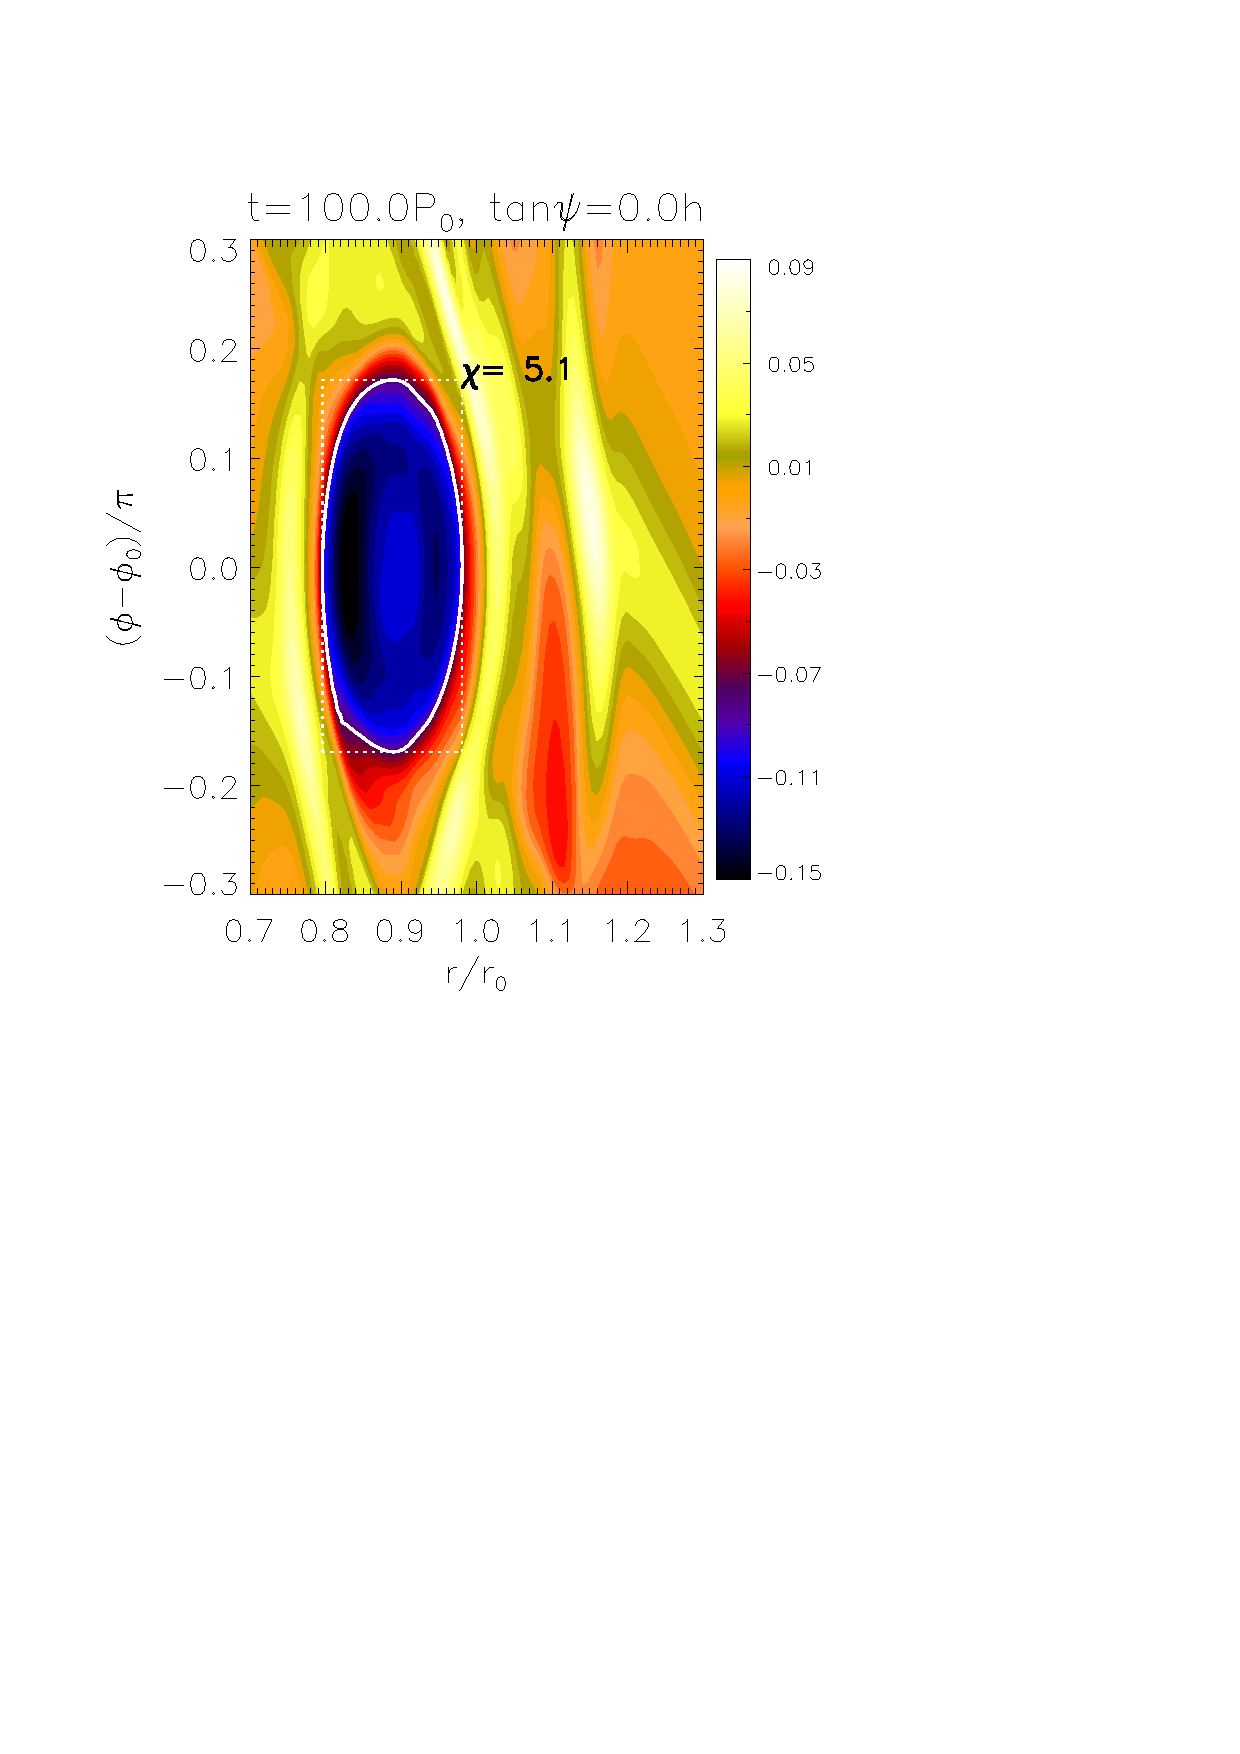
\includegraphics[scale=.27,clip=true,clip=true,trim=2.3cm
     0.cm 0cm
     0.9cm]{figures/bump0_vort010}
  \caption{Evolution of the inviscid case B0. Top: midplane density fluctuation, 
    $\Delta\rho(z=0)$. Bottom: midplane
    Rossby number (note the different axis range from the top plots). 
    Here, $\chi$ is an empirical measure of the final vortex
    aspect-ratio. $\phi_0$ is the azimuth of 
    $\mathrm{max}\left[|\Delta\rho(z=0)|\right]$
    \label{bump0_bump1}}
\end{figure}

\subsubsection{The effect of a viscous layer}
We now examine viscous cases V0 --- V3. Recall  
from Table \ref{artificial_bump} that the 
thickness of the upper viscous layer increases from case V0 to case
V3. At the reference radius, the viscous layer (with $
\hat{\nu}\sim10^{-4}$) occupies the uppermost $0\%,\,25\%,\,50\%$ and
$100\%$ of the vertical domain for cases V0, V1, V2 and V3,
respectively.    

We first compare the control case V0 to the fiducial
inviscid case B0. Table \ref{artificial_bump} shows that despite
increasing the viscosity by a factor of $10^3$, the change to the
linear mode frequencies are negligible in going from case B0 to
V0. The value of $a_m$ and minimum Rossby number show that the final
vortex in V0 is only slightly weaker than that in B0. This is also
reflected in  Fig. \ref{bump0_bump1} (case B0) and the left most column of
Fig. \ref{vdamp0} (case V0). Case V0 develops a more elongated 
vortex with smaller $|\Delta\rho|$ than that in case B0. 
  
As we increase the thickness of the viscous layer from case V0 to V3, 
Table \ref{artificial_bump} shows the dominant linear mode remains at
$m=4$, but linear growth rate does appreciably decrease 
(by $\sim 34\%$ from case V0 to V3). However, these linear growth timescales
are still $O(P_0)$.  
We have the important result that the effect of viscosity on the
instability through the linear perturbations is not significant as the
RWI remains dynamical even in the high viscosity disc.   %linear
                                %perturbations not effecitvely damped out

%replace with energy discussion 
%The top row of Fig. \ref{vdamp0} show the density fluctuations of the
%viscous cases. Comparing the second column in Fig. \ref{vdamp0} (case
%V1) to the top panel (case V0), we see that introducing the
%viscous layer lengthens the lifetime of the density perturbation in the
%nonlinear regime, since $\max(\Delta\rho)\simeq 0.47$ is maintained for
%the second half of the simulation for case V1, but this value decreases
%by about 0.1 for case V0 over the same timescale. 

Increasing the viscous layer further to case V2 and V3, we observe an
increase in the dominant azimuthal wavenumber in the nonlinear phase
(third and fourth columns in the top row of Fig. \ref{vdamp0}).  While
$\max(\Delta\rho)$ decreases with increasing viscosity, its
distribution becomes more global.  

\begin{figure*}
   \centering
   \includegraphics[scale=.39,clip=true,trim=0cm 0.9cm 0cm
     0.99cm]{figures/vdamp0_pdisk010}\includegraphics[scale=.39,clip=true,trim=2.3cm
     0.9cm 0cm
     0.99cm]{figures/vdamp2_pdisk010}\includegraphics[scale=.39,clip=true,trim=2.3cm 
     0.9cm 0cm
     0.99cm]{figures/vdamp3_pdisk010}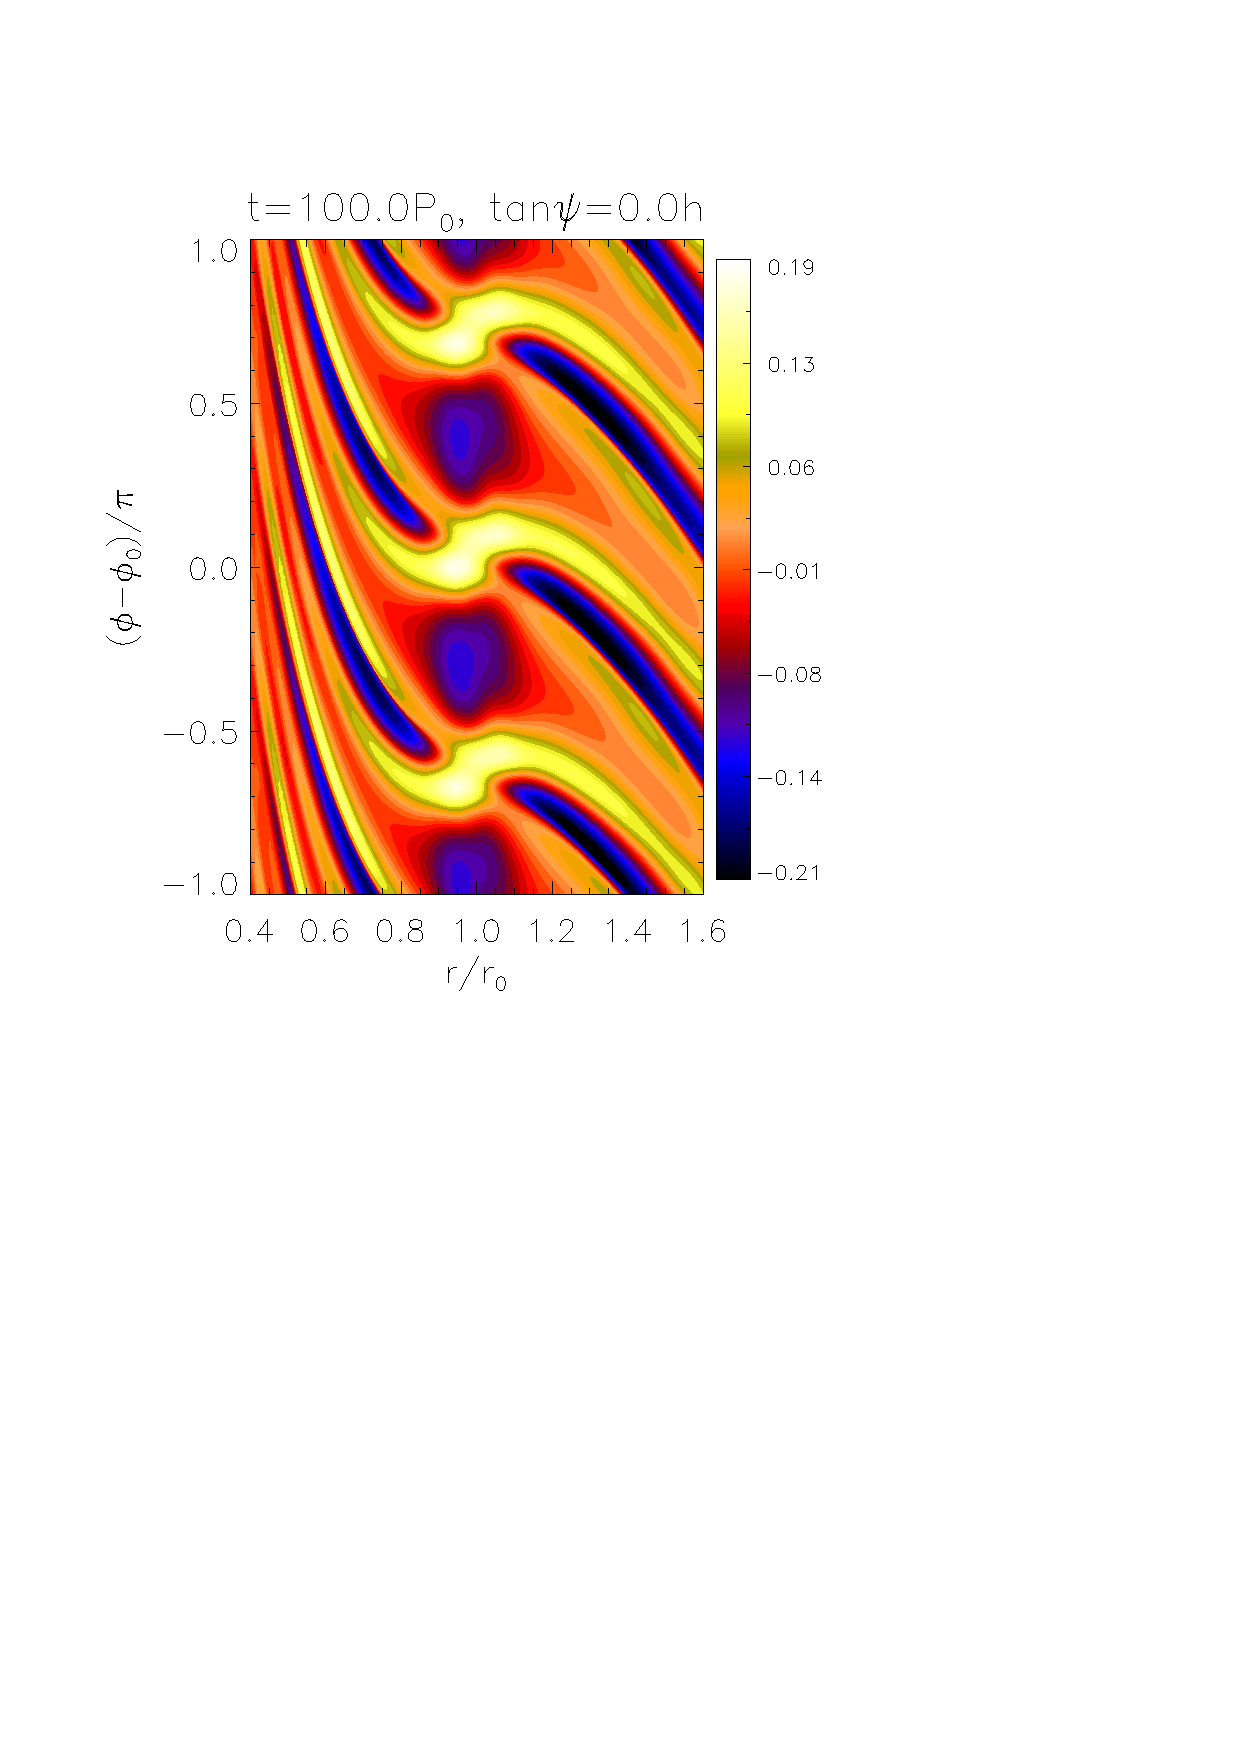
\includegraphics[scale=.39,clip=true,trim=2.3cm
     0.9cm 0cm
     0.99cm]{figures/vdamp0_nu4_pdisk010}\\
      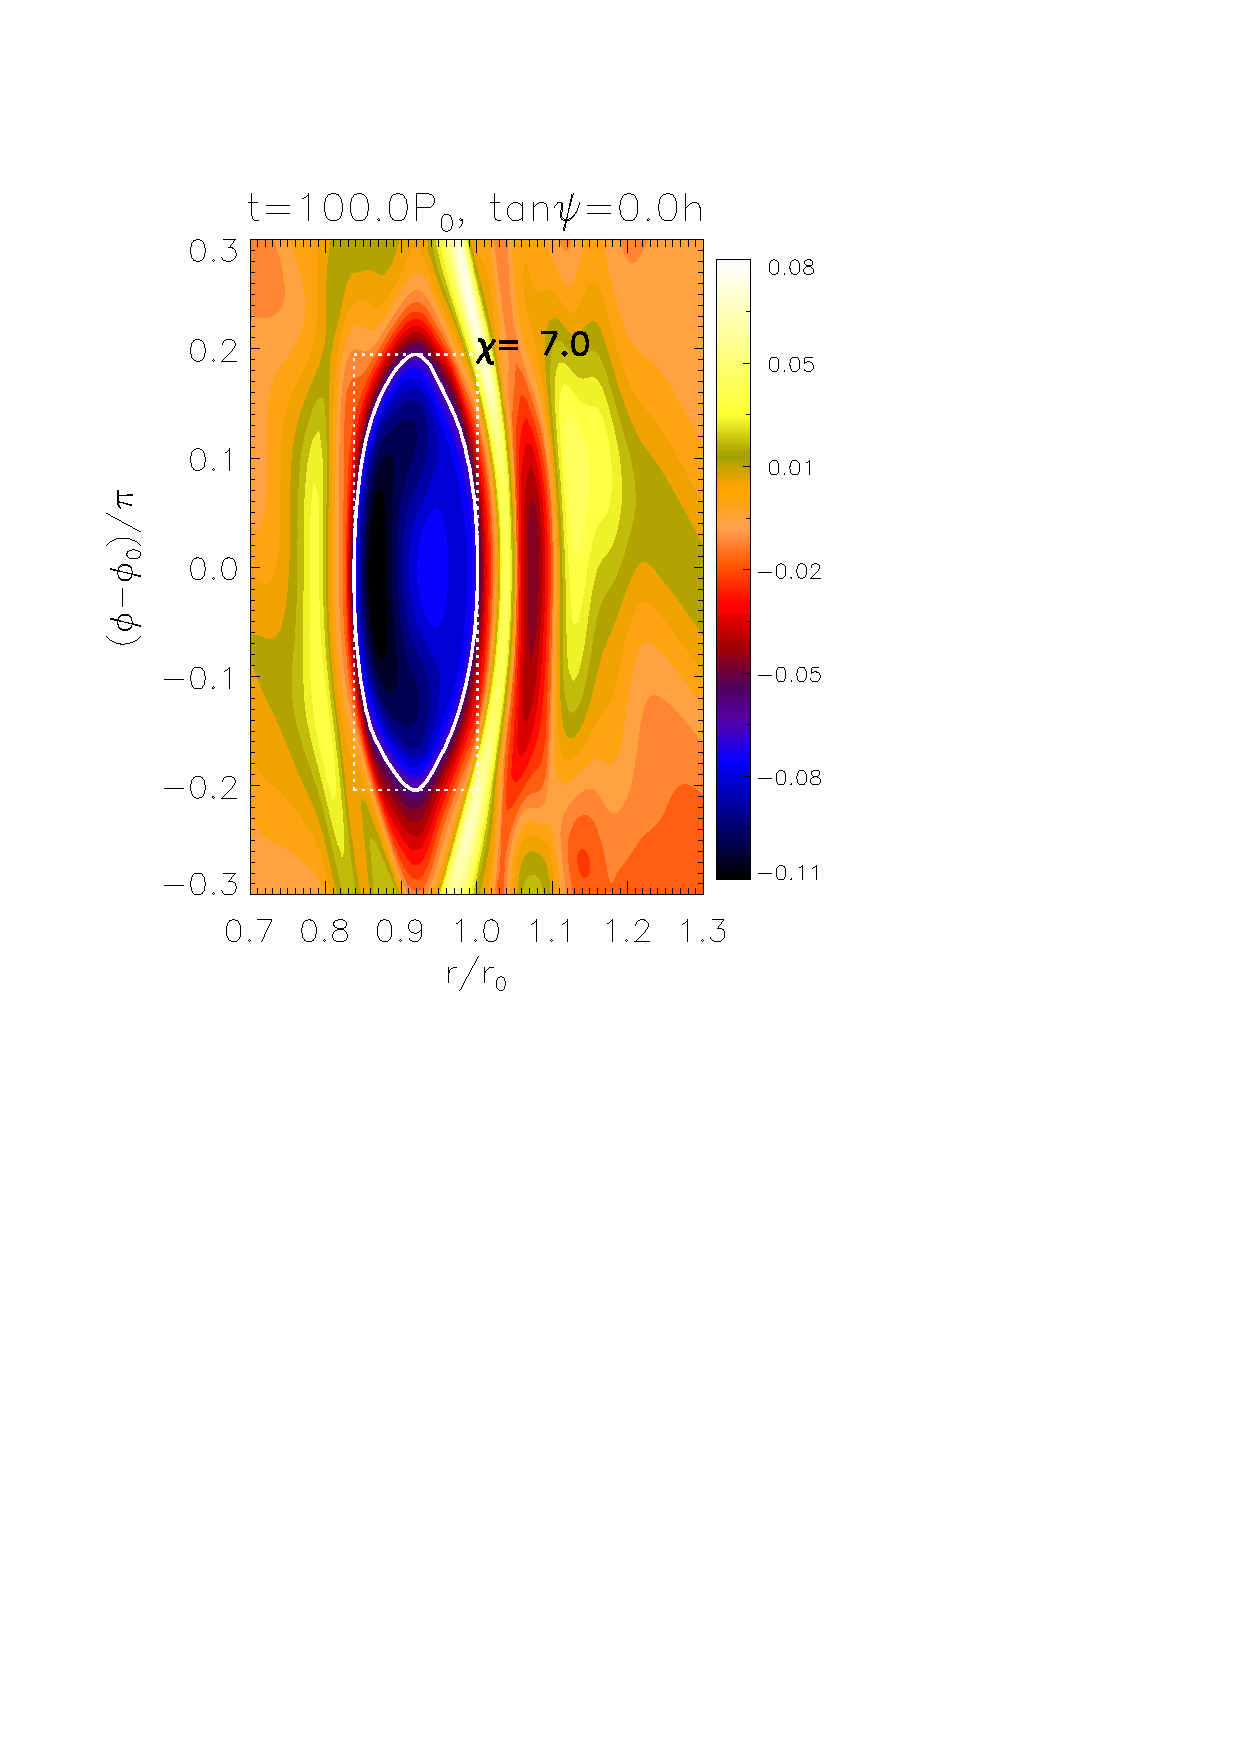
\includegraphics[scale=.39,clip=true,trim=0cm 0.cm 0cm
     0.99cm]{figures/vdamp0_vort010}\includegraphics[scale=.39,clip=true,trim=2.3cm
     0.0cm 0cm
     0.99cm]{figures/vdamp2_vort010}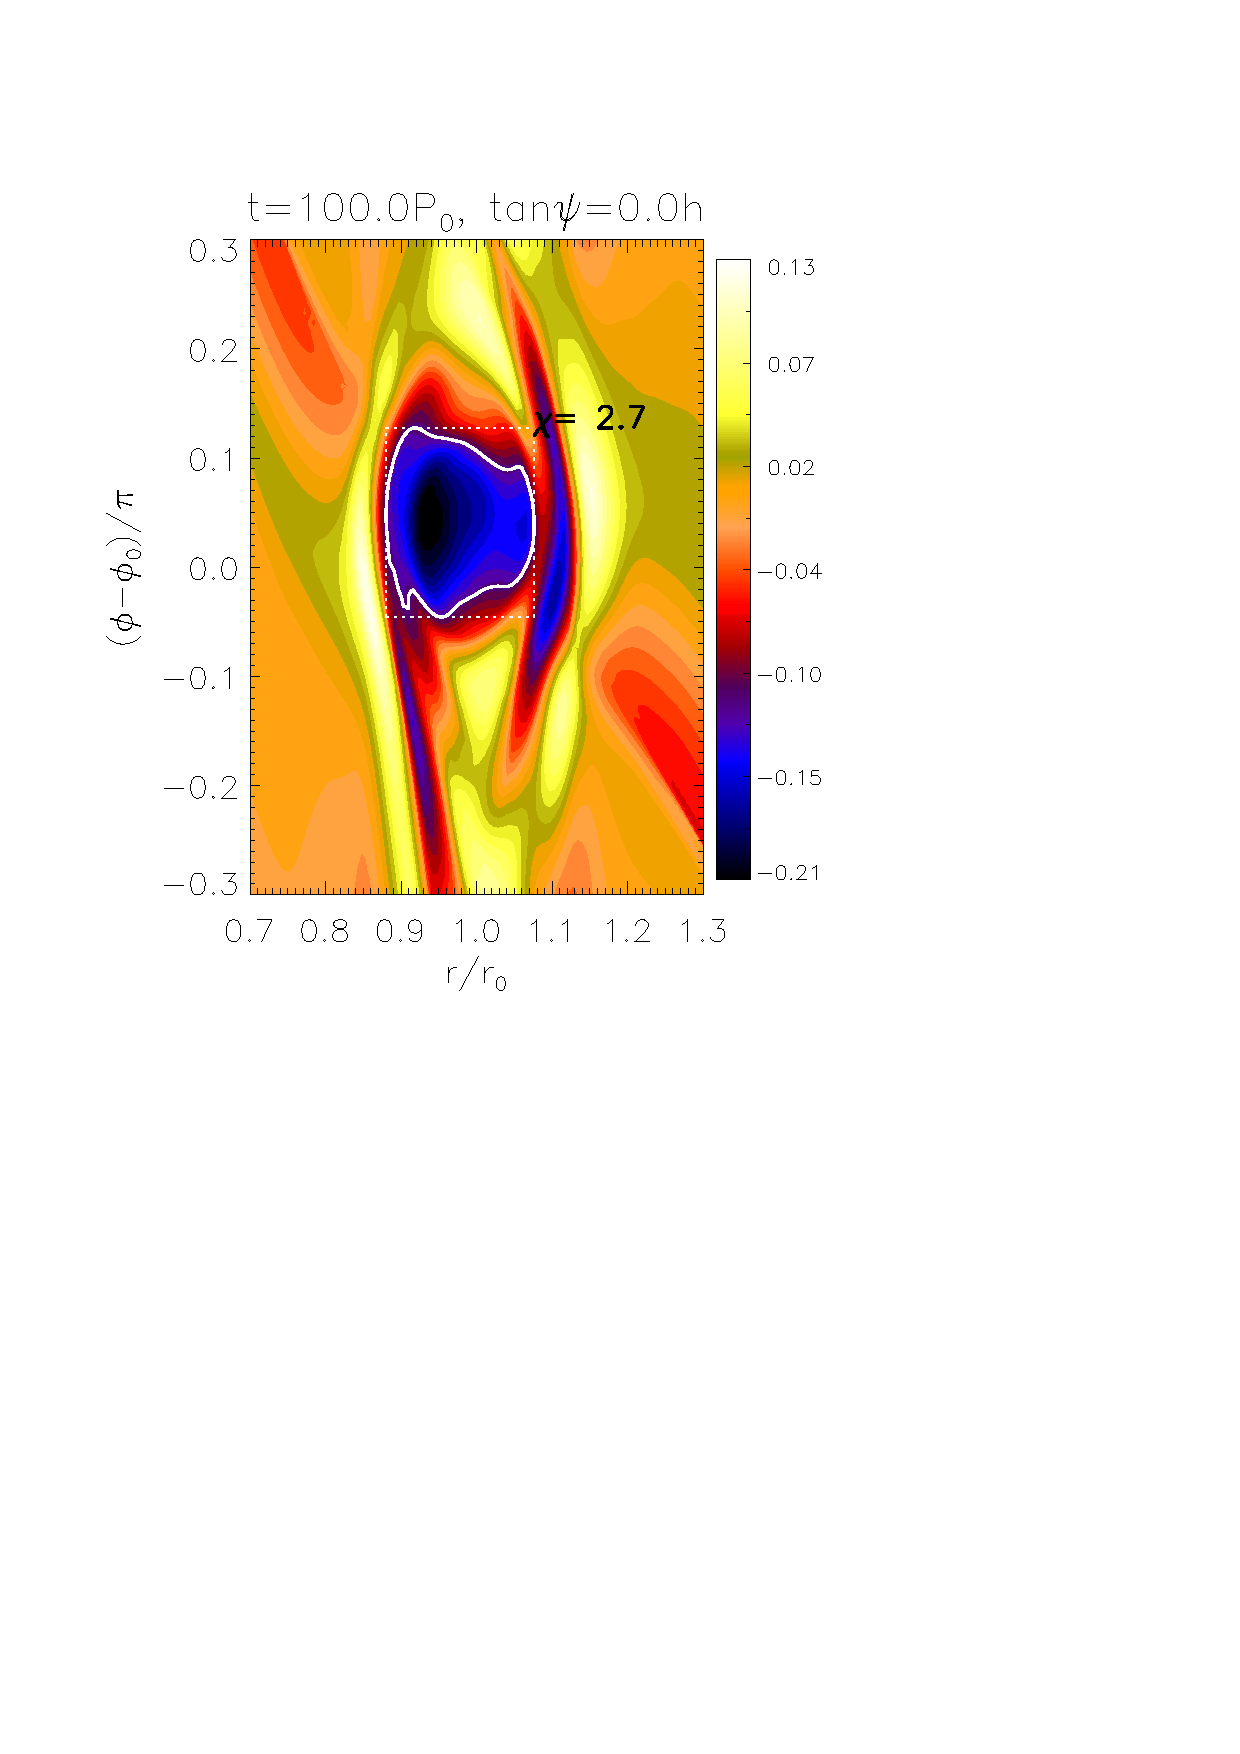
\includegraphics[scale=.39,clip=true,trim=2.3cm 
     0.0cm 0cm
     0.99cm]{figures/vdamp3_vort010}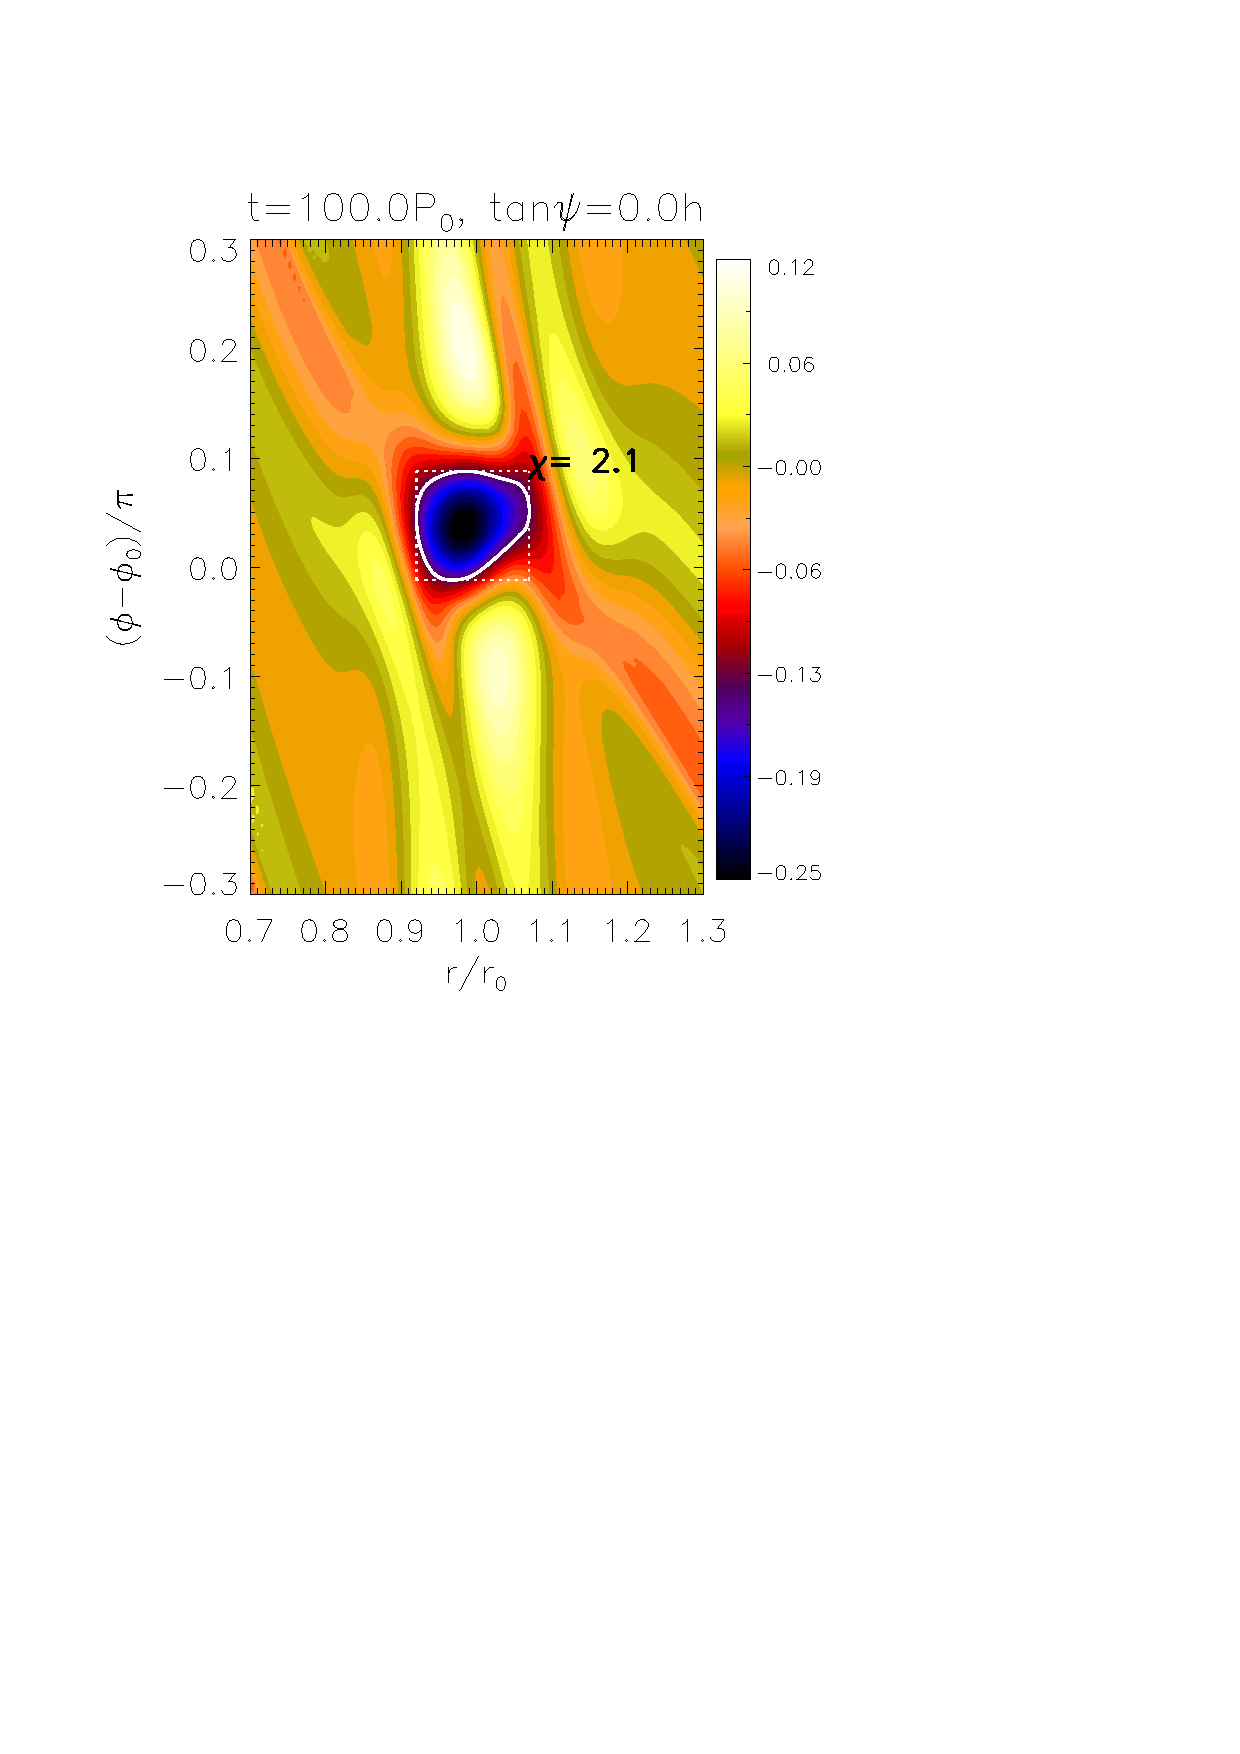
\includegraphics[scale=.39,clip=true,trim=2.3cm
     0.0cm 0cm
     0.99cm]{figures/vdamp0_nu4_vort010}
   \caption{Vortex formation in viscous discs initialised with
     artificial density bumps. Snapshots are taken at $t=100P_0$. The
     thickness of the viscous layer increases from left to 
     right: case V0, V1, V2 and V3.  
     Top: non-axisymemtric density field at the midplane
     $\Delta\rho(z=0)$. Bottom: midplane Rossby number
     $Ro(z=0)$. Here, $\phi_0$ is the azimuth of $\max[\Delta\rho(z=0)]$. 
     \label{vdamp0}
   }
\end{figure*}

Fig. \ref{vdamp0_vort} compares the Rossby number associated with the
over-densities produced by the RWI. Thickening the viscous 
layer decreases the vortex aspect-ratio. Since their widths remain
at $\sim 2H_0$, the vortices become smaller with increasing
viscosity. This may be partly attributed to fewer vortex merging
events having occured as viscosity is increased. The merging of
two vortices usually leads to a larger but weaker vortex (smaller
$|Ro|$), so if vortex merging is resisted then each vortex may evolve
separately. Vortices then become stronger as viscosity is increased
(more negative $Ro$).



%Notice the difference between the snapshots taken at $t=50P_0$ and at
%$t=100P_0$ in Fig. \ref{vdamp0}---\ref{vdamp0_vort}
%diminishes with increasing viscosity. In fact, we found the
%high-viscosity case V3 reached steady-state after $t\geq40P_0$. Thus,
%with increasing viscosity the system resists nonlinear vortex merging
%evolution is halted  
%to produce a single vortex, which usually occurs on a dynamical
%timescale in inviscid simulations (case B0). 

%%%%%%%%%%%%%%%%%%%%%%%%%%%%%%%%%%%%%%%%%%%%%%%%%%%%%%%%%%%%%%%%%%%%


\subsection{Order of magnitude comparison of timescales}
The observation of stronger vortical structures (more negative $Ro$
and smaller vortex aspect-ratio) with increasing
viscosity is unexpected, since one normally expects viscosity to
smooth out the flow. We can make sense of this result by comparing key
timescales relevant to the problem. 

The characteristic spatial scale of the background density bump and of
the instability is the local scale-height $H$, so the associated
viscous timescale is    
\begin{align}
  t_\nu = \frac{H^2}{\nu}\sim \frac{h^2}{\hat{\nu}\Omega}. 
\end{align}
The linear instability growth timescale is
\begin{align}
  t_\mathrm{RWI} = \frac{1}{\epsilon \Omega},
\end{align}
where $\epsilon$ is found from numerical simulations. 
The ratio of these timescales is
\begin{align}
  \frac{t_\nu}{t_\mathrm{RWI}} \sim \frac{\epsilon h^2}{\hat{\nu}}.
\end{align}
Table \ref{artificial_bump} indicates $\epsilon \sim 0.1$. 
Inserting $h=0.1$ and $\hat{\nu}=10^{-4}$ gives $t_\nu \sim 10
t_\mathrm{RWI}$. That is, viscosity damping is slower than linear
growth, even for the highest viscosity values we consider. The linear
phase of the instability is therefore unaffected by viscosity. 

\cite{meheut13} argued that $t_\mathrm{RWI}$ is also the vortex
turn-over time $t_\mathrm{turn}$ when the instability saturates and
the linear phase terminates. Then 
$t_\nu\sim 10 t_\mathrm{turn}$, implying viscous effects 
are unimportant over a turn-over time. 
However, if we estimate a vortex turn-over time as $t_\mathrm{turn}
\sim 2\pi/|Ro|\Omega$ then $t_\nu\sim (h^2|Ro|/2\pi\hat{\nu})t_\mathrm{turn}$.  
Inserting $h=0.1,\,\hat{\nu}=10^{-4}$ and $|Ro|=0.25$ (case V3) gives 
$t_\nu \sim 4t_\mathrm{turn}$. Therefore, depending on the vortex shape, 
$t_\nu$ may not be much larger than $t_\mathrm{turn}$. 

%% \cite[The inequality accounts for the fact that the
%% turn-over time is longer for more elogated vortices,][]{lesur09}. 
%Similarity between $t_\nu$ and $t_\mathrm{turn}$ suggest viscosity
%should have smoothed out the vortical structure. 

In any case, our simulations span several local viscous time-scales,
$t_\mathrm{sim}\sim 10t_\nu $, so viscous damping should
have taken place. On the contrary, $Ro$ becomes more negative as the
viscous layer increases from case V0 to V3. To rationalise this
observation, we recall that the RWI is fundamentally
associated with a vortensity minimum and the instability is stronger
for deeper minima \citep{li00}.  
%and the viscosity profile has been specially chosen to
%maintain such a structure in a steady state in the absence of
%perturbations.  

\subsection{Potential voritcity evolution}
Consider the potential vorticity perturbation at the bump radius, which was
found to be  
\begin{align}\label{vortensity_pert}
  \left.\frac{\aziavg{\eta_z}(t=100P_0)}{\eta_z(t=0)}\right|_{R=r_0} - 1 = 
  \begin{cases}
    3.99  & \text{Case V0} \\
   3.03  & \text{Case V1} \\
   2.24  & \text{Case V2} \\
   1.71  & \text{Case V3} \\
  \end{cases}.
\end{align} 
(This value is 4.92 for the inviscid case B0.) The PV
perturbation is positive, so the initial PV minimum is weakened
by the vortices \citep{meheut10}. This effect
diminishes with increasing viscosity. One contributing factor is 
that viscosity reduces the linear growth rate, implying the linear
perturbations saturate at a smaller amplitude \citep{meheut13}. This
is expected to weaken the background axisymmetric structure to a lesser
extent.    

We also recall that in the present simulations, the time-independent
viscosity profile was specially chosen to be consistent with a
steady-state disc containing a localised PV minimum.  
That is, the viscosity profile is also radially structured. We suggest
that for such setups, viscosity attempts to restore the initial disc
profile, i.e. the initial PV minimum.   

When viscosity is small, the viscous timescale is long compared to our
simulation timescale. In this case the nonlinear evolution of the
instability---vortex formation---weakens the PV minimum with viscosity
playing no role. As we increase viscosity, the viscous timecale
associated with the density bump becomes shorter than our simulation
timescale. %deviations away from the initial bump is smoothed out by
            %viscosity 
This means that over the course of the simulation, our spatially-fixed
viscosity profile acts as a source of PV minimum. 

In essence, in the nonlinear regime there is competition
between destruction of the background PV minimum by the
vortices and reformation of the initial radial PV minimum by the
imposed viscosity profile. We except this latter to support the
instability, leading to stronger vortices.  

 
We point out that the snapshots in
Fig. \ref{vdamp0}---\ref{vdamp0_vort} are taken at the midplane, but  
the influence of viscosity is apparent even when comparing case V1 to
V0, i.e. when the viscous layer is confined near the upper
boundary. This demonstrates the vertically-global nature of vortex
formation through the RWI. Conditions near the disc
surface should be expected to influence the instability throughout the
fluid column. 




\section{Vortex formation at planetary gap edges in layered
  discs}\label{disc-planet} 
The previous simulations, while necessary to isolate the effect of 
viscosity on the linear RWI, has the disadvantage that the radially
structured viscosity profile may act to source radial disc structure
in the non-linear regime. In this section, we use disc-planet interaction to
create the disc structure required for instability, and employ a radially smooth
viscosity profile. We therefore expect viscosity to only
act as a damping mechanism. 

Vortex formation at gap edges is seen in many  
2D and 3D hydrdynamical simulations of giant planets in low viscosity discs 
\citep{valborro07,lin10,lin11a,lin12}. The fact that this is due to
the RWI has been explicitly verified through linear stability
analysis of planetary gap profiles produced from 2D simulations
\citep{valborro07,lin10}. Here, we simulate gap-opening giant planets
in 3D discs where the kinematic viscosity varies with height above the
disc midplane. Our numerical experiments are similar in spirit to
those performed by \cite{pierens10}, but our focus here is gap
stability in a layered disc. 
 
\subsection{Radially smooth viscosity profile for disc-planet
  interaction}\label{planet_visc_mode} 
Using the same notation as \S\ref{visc_model}, we impose a viscosity
profile $\hat{\nu}$ such that 
\begin{align}\label{planet_visc_profile}
  \hat{\nu}\Sigma_i(R)=%\frac{d\ln{\Omega_i}}{d\ln{R}} =
  \hat{\nu}_0\left[1+Q(\psi)\right]\Sigma_i(r_0)%\left.\frac{d\ln{\Omega_i}}{d\ln{R}}\right|_{r_0}.      
\end{align}
We have set the dimensionless argument in Eq. \ref{step} to
$\zeta=\psi$. Recall $\psi=\pi/2-\theta$ is the angular height away from the midplane. 
The viscosity increases from its floor value $\hat{\nu}_0$ by a factor
$A_\nu$ for $\psi > \zeta_\nu$. So the viscous layer is 
a wedge in the meridional plane, which conveniently fits into our
spherical grid. %Note that setting $\psi = 0$ in Eq. \ref{planet_visc_profile} gives
%the appropriate viscosity profile for a razor-thin viscous disc in
%steady state when the initial cylindrical radial velocity 
%is set by Eq. \ref{init_vr}. 

The typical viscosity value adopted for disc-planet simulations, 
$\hat{\nu}\sim 10^{-5}$ or $\alpha\sim 10^{-3}$, is known to surpress
vortex formation in 2D \citep{valborro07, mudryk09}. 
We therefore choose a floor viscosity of $\hat{\nu}_0=10^{-6}$.
The angluar thickness of the viscosity transition is fixed to
$\Delta\zeta_\nu = 0.2h$. Fig. \ref{planet_visc2d} gives an example of this
viscosity profile. We will quote the thickness of the viscous layer as a 
percentage of the entire $\theta$ domain size. 

\begin{figure}
  \centering
  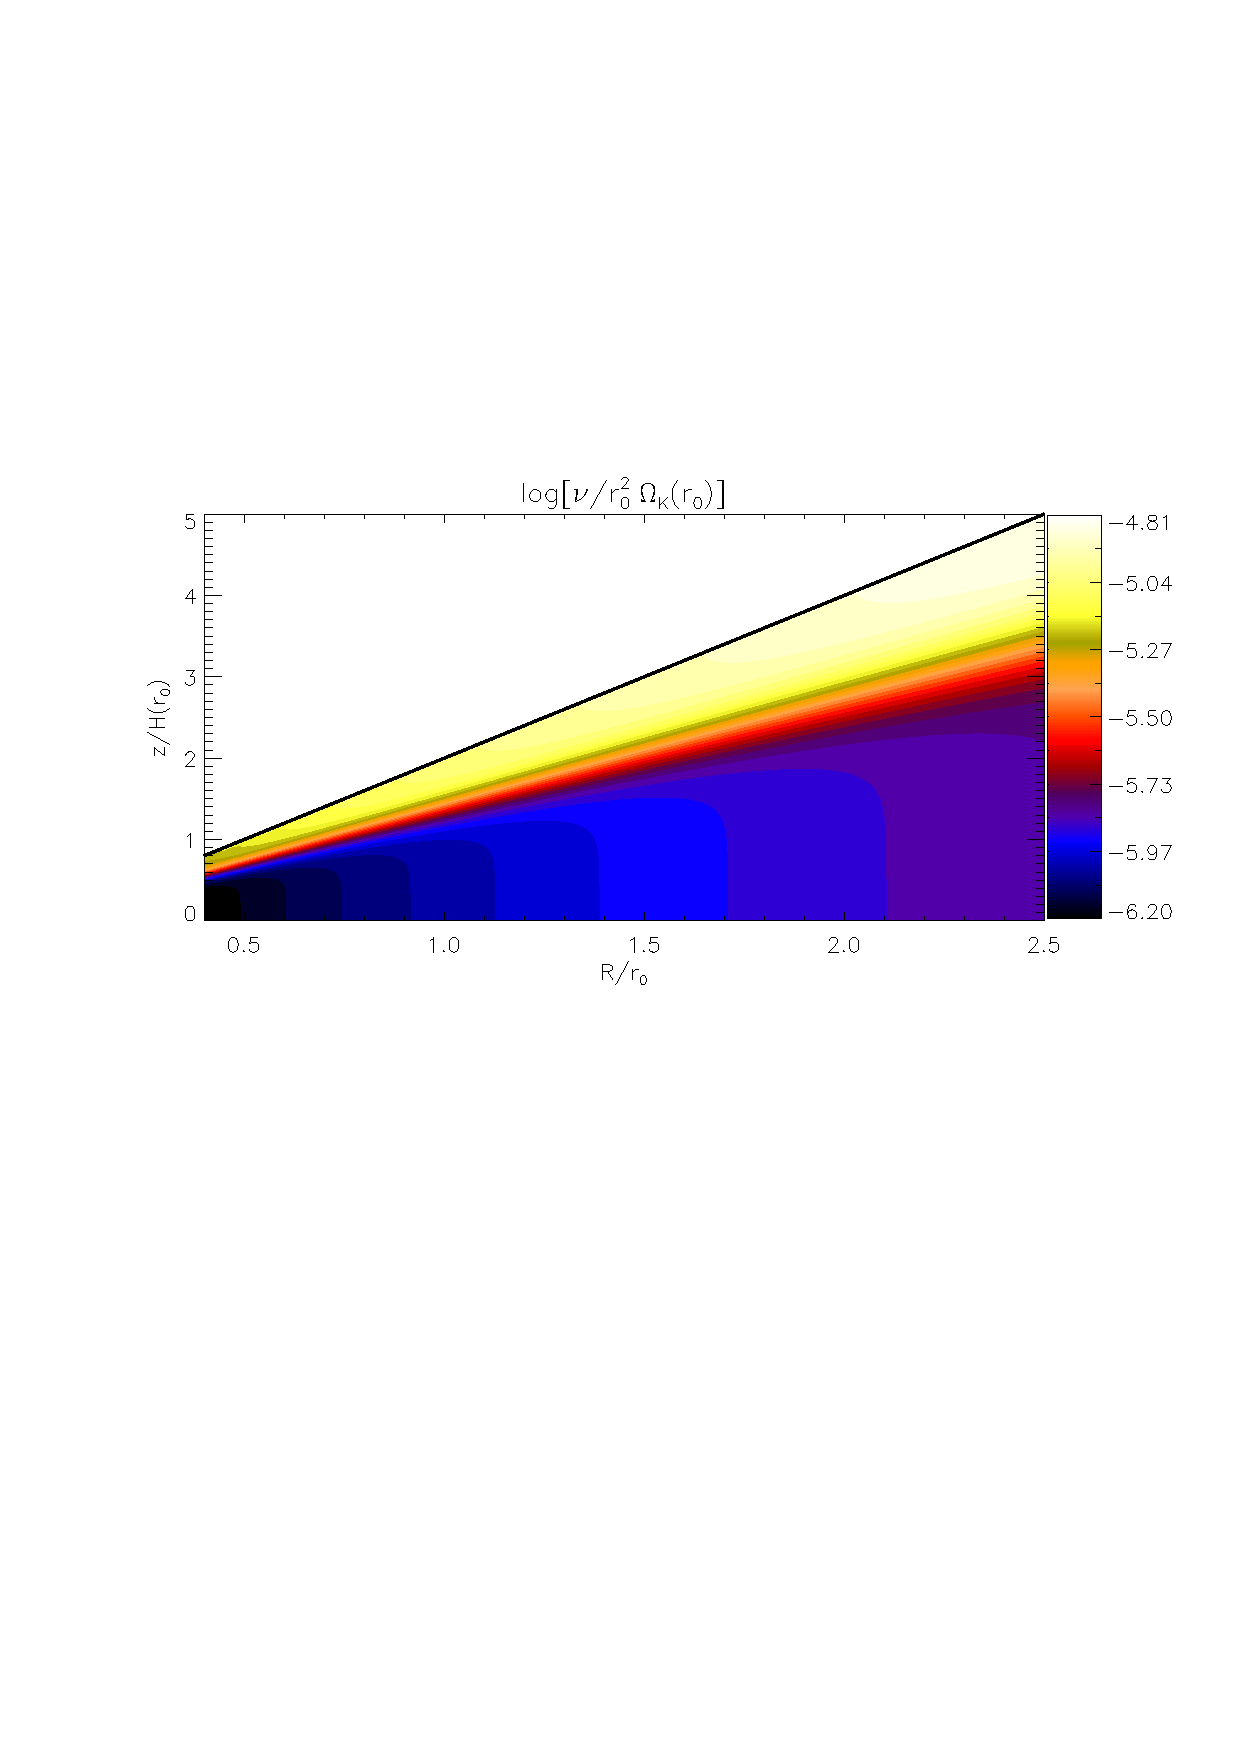
\includegraphics[width=\linewidth]{figures/pdisk_visc2d_planet}
  \caption{Example of the `wedge' viscosity profile
    imposed in disc-planet simulations
    (Eq. \ref{planet_visc_profile}).  
    For a disc with constant aspect ratio, as chosen here, the viscous
    layer occupies a constant number of scale heights across the
    radial range. This specific plot corresponds to case P1, so the
    viscous layer (yellow-white colours) always occupies the uppermost
    $H$ at each cylindrical radius. 
    The solid line
    delineates the upper boundary of the computational domain.
    \label{planet_visc2d}}
\end{figure}

%This viscosity profile is a smooth
%function of radius, meaning a localized radial density structure will
%be smoothed out, unless it is maintained by an external
%source (the planet in our case). We therefore expect viscosity to only
%act as a damping mechanism, c.f. a source for radial structure in the
%previous section. 

\subsection{Disc-planet simulations} 
We simulate locally isothermal discs with constant aspect-ratio
$h=0.05$ (by choosing $q=1$), vertical extent $n_h=3$ scale-heights 
and radial extent $[\rin,\rout]=[0.4,2.5]r_0$. Initially the surface density is smooth
($A=1$) with zero meridional velocity ($v_r=v_\theta=0$). 
%cylindrical radial velocity is given by
%Eq. \ref{init_vr}. 
The standard resolution is $(N_r, N_\theta,
N_\phi)=(256, 32n_h, 768)$, corresponding to $6,\,32,\,6$ 
cells per $H$ along the $r,\theta,\phi$ directions at the reference
radius. We apply a damping rate $\hat{\gamma}=2$ with the reference
velocity field $\bm{v}_\mathrm{ref}=(0,0,v_\phi)$ in spherical
co-ordinates.   

We insert into the disc a planet of mass  
$M_p=10^{-3}M_*$, which corresponds to a Jupiter mass planet if
$M_*=M_{\sun}$. The softening length adopted for the planet potential is
$\epsilon_p=0.5r_h$. The planet potential is switched on 
smoothly over $t\in[0,10]P_0$. We note that the disc can be considered
as two-dimensional for gap-opening giant planets, because the Hill
radius $r_h$ exceeds the local scale-height $H_0$ ($r_h/H_0\simeq1.4$
in our cases).   

We remark that the above choice of physical and numerical parameter
values are typical for global disc-planet simulations
\citep[e.g.][]{valborro06,mignone12}.   

%\subsubsection{Standard runs} 
%The fiducial vertical extent of our disc model is $n_h=2$
%scale-heights at $R=r_0$.  The control run, case P0, has $A_\nu=1$ so there is 
%no viscous layer. The kinematic viscosity is therefore
%$\hat{\nu}\sim10^{-6}$  everywhere. We then introduce a viscous
%layer (or wedge) occupying the uppermost $25\%$ and $50\%$ of the
%vertical domain in cases P1 and P2, by choosing the transition angle
%at $\zeta_\nu = 1.5h,\,1.0h$, respectively. These layers have a kinematic 
%viscosity of $\hat{\nu}\sim 10^{-5}$ by setting $A_\nu=10$.  (See
%Fig. \ref{planet_visc2d} for the viscosity profile for case P1.)  


\subsubsection{Runs}
%We also consider two runs with an extended vertical domain size
%$n_h=3$. 

Our fiducial case P0 has $A_\nu=1$ so there is no viscous layer, thus
$\hat{\nu}\sim 10^{-6}$ everywhere. For case
P1 and P2 we set $A_\nu=100$ with transition angle $\zeta_\nu=2h$ and
$h$, respectively. Thus the viscous layer with $\hat{\nu}\sim10^{-4}$
occupies the upper $H$ and $2H$ of the vertical domain. We also
consider case P0.5, in which we resume case P0 from 
$t=100P_0$ but with the layered viscosity profile of case P1. 

%Thus, the viscous layer with $\hat{\nu}\sim10^{-4}$ occupies $33\%$ of
%the uppermost vertical domain. %Note that most of the mass is contained
%in the low viscosity layer. 
%We also consider case P6 without a
%viscous layer but 


%%%%%%%%%%%%%%%%%%%%%%%%%%%%%%%%%%%%%%%%%%%%%%%%%%%%%%%%%%%%%%%%%%%%%%%%%%%%%%%


\subsection{Results}
Our disc-planet simulations are summarised in Table \ref{planet_sims}.
We focus on vortex-formation at the outer gap edge. 
The non-axisymmetric mode amplitude in the last column was 
averaged over the shell $r\in[1.2,1.6]r_0$ and over time 
$t\in[100,150]P_0$. We examine the $m=1$ mode since 
for non-self-gravitating planetary gaps, if unstable, usually develop
a single vortex in quasi-steady state \citep{valborro07,lin10}.   

%for  mode amp: spatial average over [1.2,1.6], time average over [100,150]P_0

\begin{table}
  \centering
  \caption{Summary of disc-planet simulations. These runs employ the
    `wedge' viscosity model described by
    Eq. \ref{planet_visc_profile}. The thickness of the viscous layer
    is measured from the upper disc boundary. Case P0.5 employs the
    viscosity profile of P0 (P1) for $t\leq100P_0$ ($t\geq100P_0$). }
    \begin{tabular}{lcccr}
      \hline\hline
      %      \multicolumn{6}{c}{\phantom{stuff}} &
      %      \multicolumn{3}{c}{Linear phase ($t\leq10P_0$)}&
      %      \multicolumn{3}{c}{$t=100P_0$}\\
      %      \cline{7-9}\cline{10-12}
      Case & $A_\nu$ &$\zeta_\nu/h$ & visc. layer& $10^2\overline{a}_1$ \\ 
      \hline
      P0      &    1     &    $\infty$      & 0     &       \\
      P0.5    &    1$\to$100 & $\infty\to2.0$ &$0\to H$ &     \\
       P1      &    100   &    2.0      & $H$   &       \\ 
      P2      &    100   &    1.0      & $2H$  &         \\ 
      \hline
  \end{tabular}
\end{table}

%\subsubsection{}

%We now consider appending a viscous layer on top of the fiducial 
%case P0. 
Case P3 is the same as case P0 above, except with an increased
vertical domain size of $3H$ at the reference radius. Case P4 has a high-viscosity layer with
$\hat{\nu}\sim10^{-4}$ in the the uppermost scale-height of the
computational domain. In other words, the bulk of the 
%% has a viscosity $\hat{\nu} \sim 10^{-5}$ and $\hat{\nu}\sim 10^{-4}$
%% for cases P3 and P4, respectively. 
disk for case P4 has a low-viscosity of $\hat{\nu}\sim10^{-6}$, but
with a viscous atmosphere appended on top.  

Fig. \ref{jup0_3h} shows the density pertubation at $t=100P_0$ for
cases P3 and P4. Case P3 is essentially identical to case P0, so the 
vortex instability is not affected by vertical domain size. We note
that the viscosity is increased in the disc atmosphere, where the
density is a factor $\sim 7$ times smaller than the midplane (but the
viscosity is $100$ times larger). The viscous layer has surpressed
vortex formation. This implies that vortex formation via
the RWI at planetary gap edges can not tolerate a signigicantly
viscous atmosphere, even if such a layer only occurs away from the
midplane.    

\begin{figure}
   \centering
%   \includegraphics[scale=.39,clip=true,trim=0cm 1.84cm 0cm
%     0cm]{figures/jup0_3h_pdisk010}\includegraphics[scale=.39,clip=true,trim=2.3cm
%     1.84cm 0cm
%     0cm]{figures/jup1_3h_pdisk008}
   \caption{Density perturbation $\delta\rho$ at the end of the
     disc-planet simulations case P3 (left, no viscous layer) and P4
     (right, viscous layer occupies $33\%$ of the uppermost vertical
     domain).   
     \label{jup0_3h}}
\end{figure}
 


%\subsection{Locally isothermal simulations}

%%\section{Discs with radial viscosity transitions}\label{dead}
Vortex-formation in at dead zone can boundaries in protoplanetary
discs ca be modeled by imposing a radially-structured viscosity
profile \citep{varniere06,crespe11} in  hydrodynamic simulations, or
more recently by directly simulating a magenised disc with a
radially-structured resistivity \citep{lyra12}. These disc models are
either 2D or unstratified 3D,  implying the transition occurs at a
fixed cylindrical radius independent of height. Vortices observed in
such simulations have been attributed to the RWI, presumably because
of the PV extremum that results from mass build-up at the (effective)
viscosity jump. No corresponding linear stability
calculations have been performed to date, however, since the `basic
state' is time-dependent.       

In this section, we generalise the above studies by  
introducing viscous layers. We explore vortex formation at the
radial boundary between of high/low viscosity regions of the disc, 
when there exsists a vertical viscosity transition as well.     

\subsection{Radially and vertically structured viscosity profile}
We adopt a similar viscosity profile as used for disc-planet
simulations, but modify it by a radial smooth-step function $f(R)$, 

\begin{align}\label{dead_profile}
  &\hat{\nu}\frac{\Sigma_i(R)}{\Sigma_i(r_0)}\frac{d\ln{\Omega_i}}{d\ln{R}} = 
  \hat{\nu}_0\left\{ \left[1+Q(\psi)\right]f + \left[ 1-
    f\right]A_\nu\right\}%\notag\\
  %  \phantom{\hat{\nu}\Sigma_i(R)\frac{d\ln{\Omega}}{d\ln{R}} =}
  \left.\frac{d\ln{\Omega_i}}{d\ln{R}}\right|_{r_0},\\
  &f(R) \equiv \frac{1}{2}\left[ 1 + \tanh{\left(\frac{R-r_0}{\Delta R_\nu}\right)} \right].
\end{align}
For $R>r_0$, the viscosity profile is the same as that used in the
previous section, while for $R<r_0$ the viscosity is uniform with 
$\hat{\nu}\sim A_\nu\hat{\nu}_0$. We set $\hat{\nu}_0=10^{-6}$ and
$A_\nu=10$. The radial transition width is fixed to $\Delta R_\nu =
0.5H_0$. As before the angular transition width is fixed to
$\zeta_\nu=0.2h$. An example of the viscosity profile produced by
Eq. \ref{dead_profile} is shown in Fig. \ref{visc2d_dead}.   

\begin{figure}
  \centering
  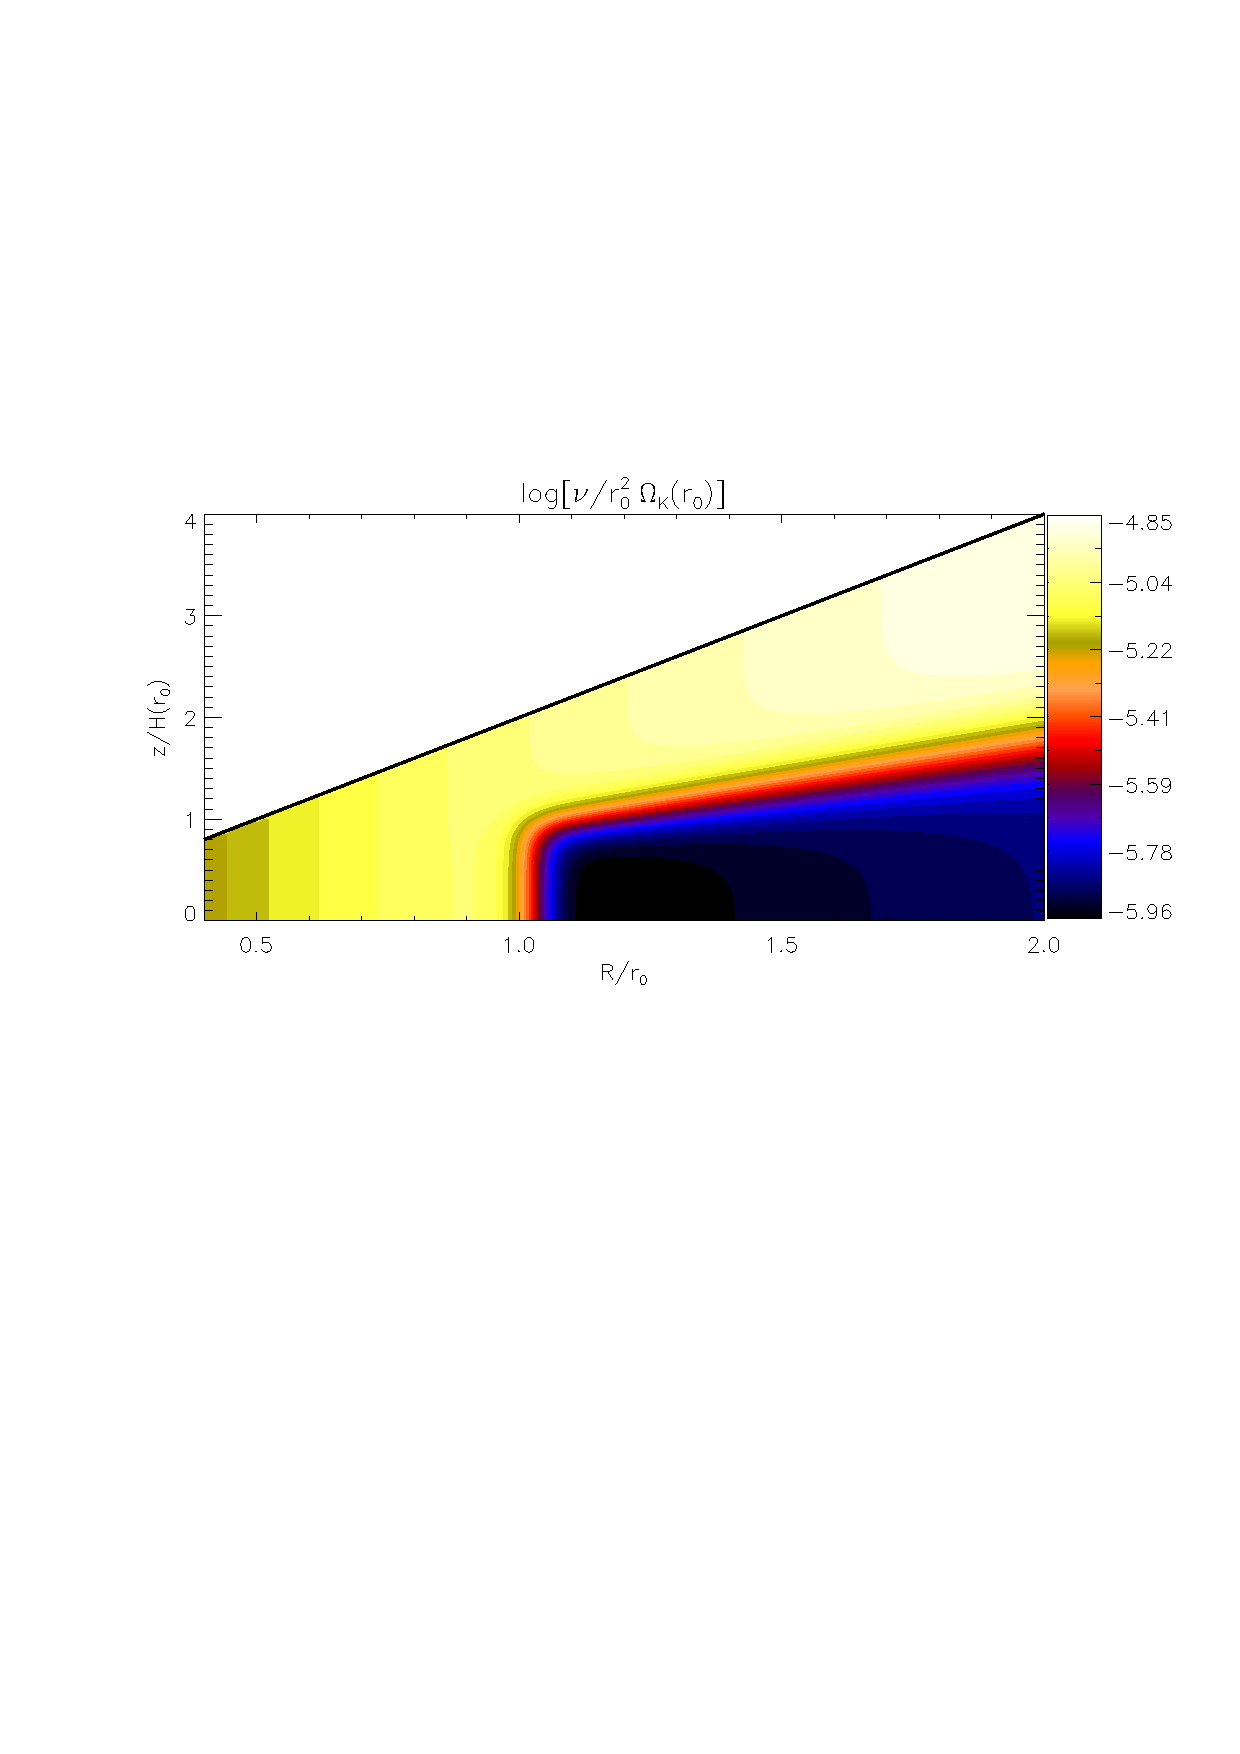
\includegraphics[width=\linewidth]{figures/pdisk_visc2d_dead}
  \caption{Example of the radially-and-vertically structured viscosity
    profile described by Eq. \ref{dead_profile}. 
    This specific plot case D2. The solid line delineates the upper
    boundary of the computational domain. 
    \label{visc2d_dead}}
\end{figure}

\subsection{Setup}
We consider discs with $h=0.1$, radial range
$[\rin,\rout]=[0.4,2.0]r_0$ and vertical size $n_h=2$. No surface
density bump is used ($A=1$). The resolution
is $(N_r,N_\theta,N_\phi)=(256,64,512)$. We initialise the disc
without radial flow, but impose perturbations to $v_r$ just after
initialisation. Note that the initial condition is not a steady-state
equilibrium solution.   

\subsection{Dead zone simulations}
Our fiducial simulation, case D0, does not have a viscous layer in the
vertical diretcion. We then consider cases D1 
and D2 with angular transitions at $\zeta_\nu=1.5h$ and
$\zeta_\nu=1.0h$, which gives a viscous layer occupying
$25\%$ and $50\%$ of the uppermost vertical domain. That is, the 
viscous layer at unit radius has thickness $0.5H_0$ and $H_0$ for
cases D1 and D2, respectively. Table \ref{dead_sims} summarises the
simulations in this section. 
 
\begin{table}
  \centering
  \caption{Summary of dead zone simulations. These runs employ the viscosity profile 
    described by Eq. \ref{dead_profile}, which invovles a viscosity
    transition both radially and vertically. The viscous layer is quoted
    as a fraction of the vertical domain at $R=r_0$. \label{dead_sims}}
  \begin{tabular}{lcccc}
    \hline\hline
    Case & $\Delta R_\nu/H_0$ & $A_\nu$ &$\zeta_\nu/h$ & visc. layer \\ 
    D0 &  0.5    &    10      &    n/a      & 0     \\%&      -0.21 \\
    D1 &  0.5     &    10     &    1.5      & $25\%$ \\% &    -0.28 \\
    D2 &  0.5     &    10     &    1.0      & $50\%$ \\%&     -0.08 \\
    \hline
  \end{tabular}
\end{table}


\subsection{Results}
To obtain an overview of disc evolution, we compare the minimum Rossby 
numbers near $R=r_0$ between cases D0, D1 and D2 in
Fig. \ref{rtrans_nuamp10_minrossby}. {\bf to be updated}.  The Rossby
number decreases when non-axisymmetric disturbances develop at
the dead zone boundary. The non-smooth evolution signifies vortex
merging. Evidently, the evolutionary timescales vary between these
cases. So we compare them at similar evolutionary stages.   

%% Cases Db0 and Db1 evolve
%% similarly, with a time-shift between them. 
%% Over the course of the simulation, both cases reach a 
%% minimum Rossby number $\sim -0.3$ at $t\simeq 120P_0,\,170P_0$ for the
%% case Db0 and Db1, respectively. We find this minima coincided with
%% vortex merging, the result being a single vortex which subsequently elongates
%% and weakens. Case Db2 evolves quite differently, it attains a minimum Rossby
%% number of $Ro\simeq-0.08$ at $t=150P_0$. This is much weaker than the
%% two previous cases, but the vortex does not weaken afterwards ($|Ro|$
%% remains roughly constant for $t\gtrsim 150P_0$).  

\begin{figure}
  \centering
  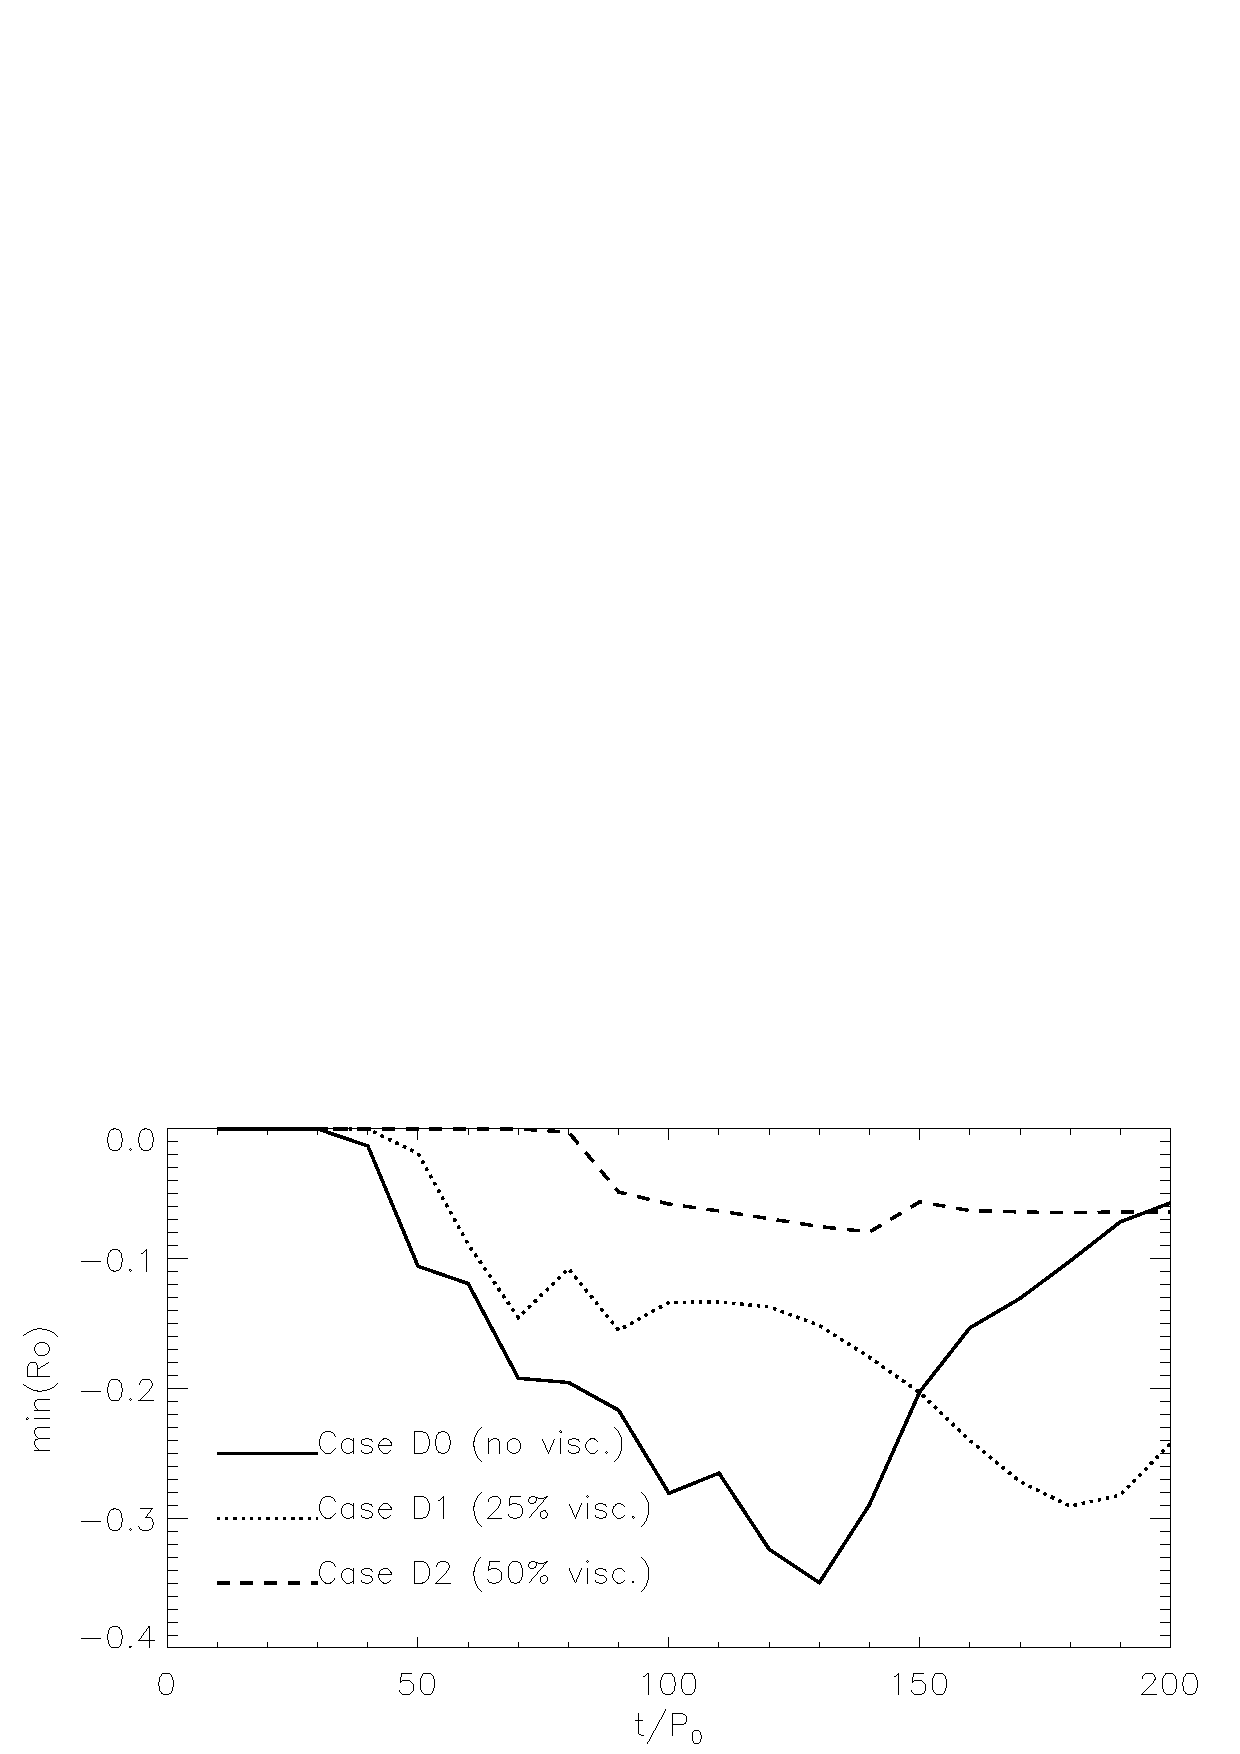
\includegraphics[width=\linewidth]{figures/rtrans_nuamp10_minrossby}
  \caption{Minimum midplane Rossby number found in case D0 (solid),
    D1, and D2 (dashed). The thickness of the viscous layer is quoted
    as the fraction of the uppermost vertical domain. 
    \label{rtrans_nuamp10_minrossby}}
\end{figure}

Fig. \ref{rtrans_nuamp10_vorten1d} shows the PV profiles as a result
of the mass build-up at the dead zone boundary. The snapshot for each
case is taken just before $Ro$ begins to decrease. 
The latter is neccessary for the RWI. We
therefore consider these profiles as the `basic state' for the
RWI. Although convenient, this is not strictly correct because the
profiles in Fig. \ref{rtrans_nuamp10_vorten1d} do not correspond to
steady states, with respect to which a linear instability is defined.   

The radial viscosity transition leads to a PV maximum and a PV minimum
on either side of unit radius. The latter is associated with the RWI. 
Case D0 and D1 have very smililar profiles, while the PV minimum is
slightly less sharp in case D2. Thus, the disc profile necessary for
instability is affected by the presence of a viscous layer. We expect
the RWI to grow more slowly in case D2 than the other cases. 

\begin{figure}
  \centering
  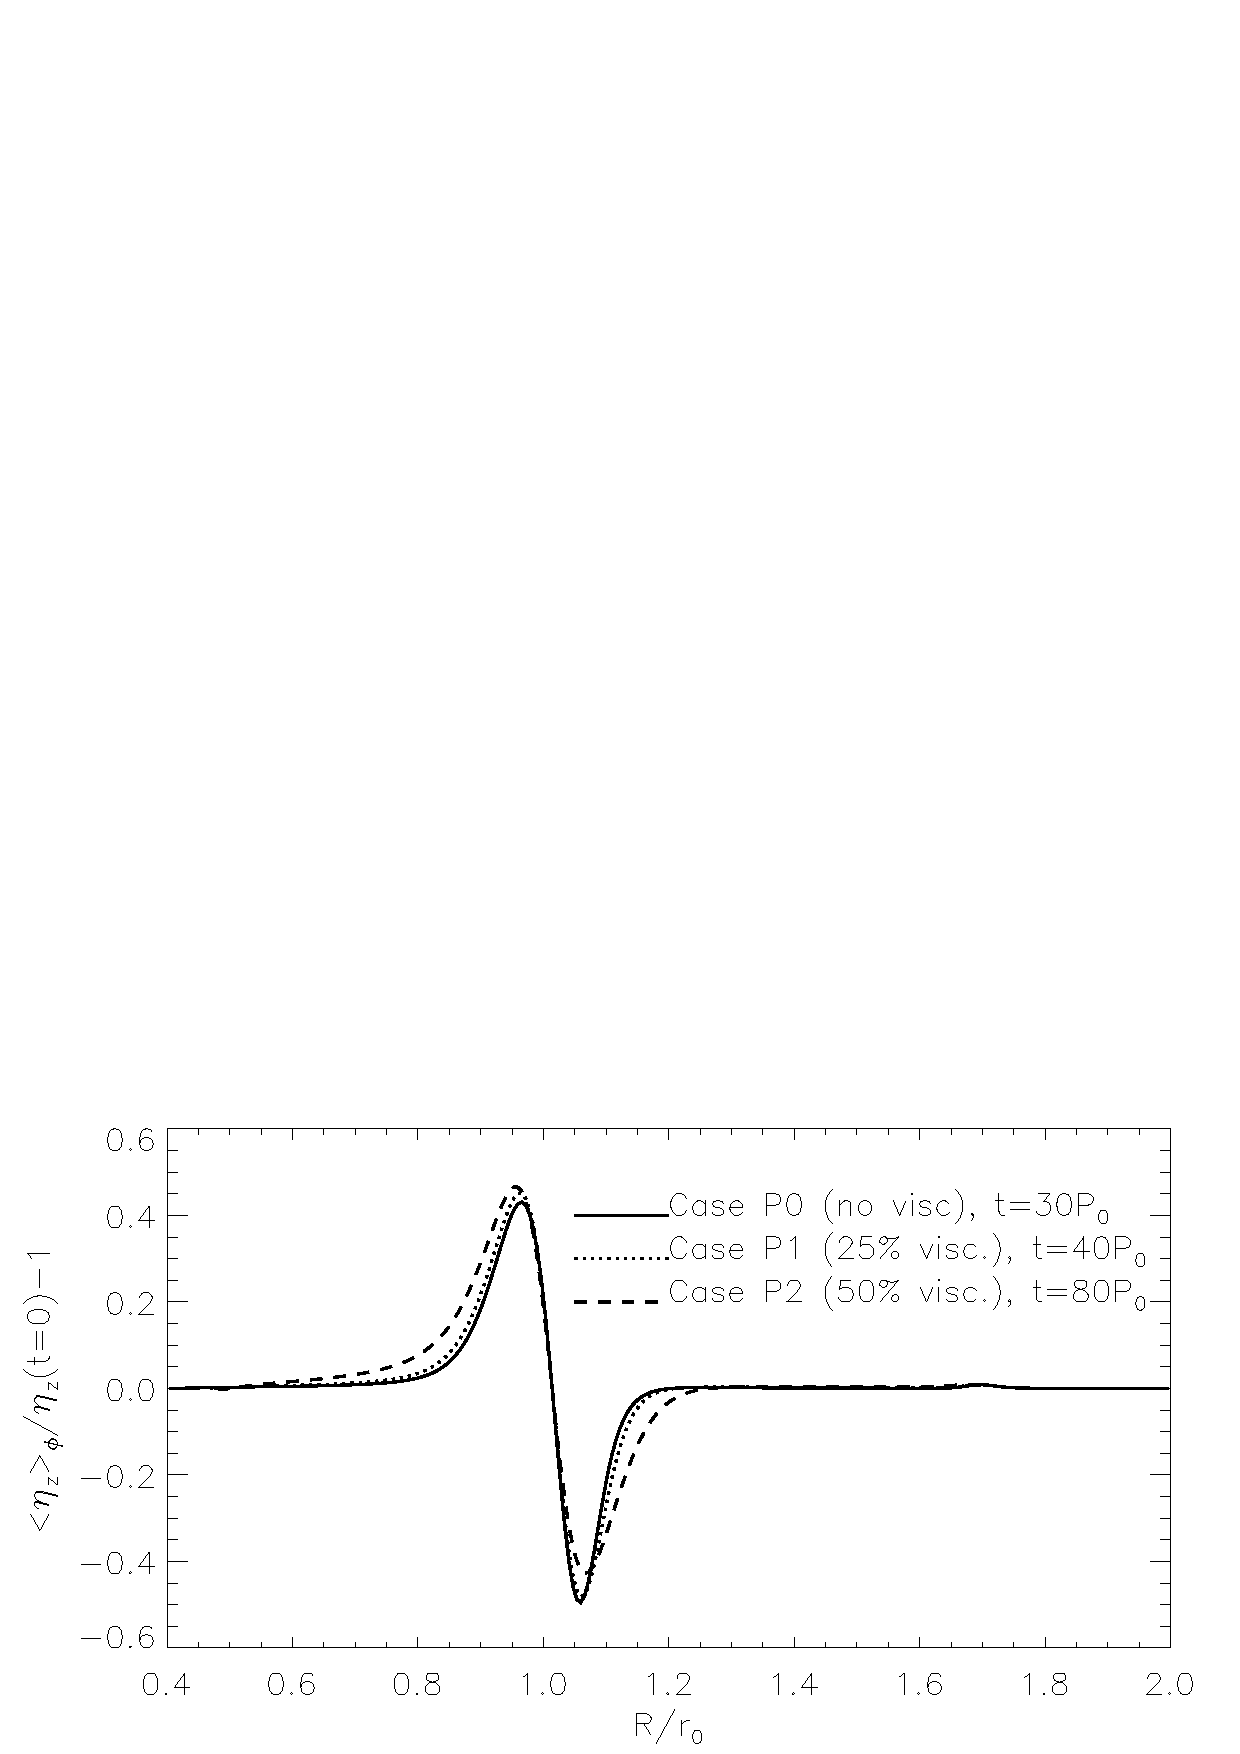
\includegraphics[width=\linewidth]{figures/rtrans_nuamp10_vorten1d}
  \caption{Potential vorticity profiles for dead zone simulations D0,
    D1 and D2. The snapshots are taken just before the Rossby numbers
    in Fig. \ref{rtrans_nuamp10_minrossby} first begins to decrease. 
    \label{rtrans_nuamp10_vorten1d}}
\end{figure}

Fig. \ref{rtrans_vdamp0_nuamp10} compares $\delta\rho$ at
$t=50P_0,\,60P_0$ and $100P_0$ for cases D0, D1 and D2, respectively.
The snapshots correspond to initial vortex formation. It is also when
the midplane $\min(Ro)$ first becomes non-negligible (see
Fig. \ref{rtrans_nuamp10_minrossby}). As expected from the PV
profiles, cases D0 and D1 are very similar, both developing the $m=3$
mode. However, case D2 develops the $m=2$ mode, because the PV extrema
is smoother. 

With the observed azimuthal wavenumbers in
Fig. \ref{rtrans_vdamp0_nuamp10}, we estimate the non-axisymmetric
mode growth rates to be $q_3\sim 0.1\Omega_0,\,0.09\Omega_0$ for cases D0 and D1; and
$q_2\sim0.05\Omega_0$ for case D2. The co-rotation radii were
%rates 0.11, 0.093 and 0.049
$r_c\sim1.073r_0,\,1.075r_0$ and $1.081r_0$, which are very close to
the radii of PV minima in Fig. \ref{rtrans_nuamp10_vorten1d}. Note
that the growth timescale is a few $P_0$, which is shorter than the
timescale to attain the PV extrema.  

\begin{figure}
   \centering
   \includegraphics[scale=.27,clip=true,trim=0cm 0.0cm 0cm
     0cm]{figures/rtrans_vdamp0_nuamp10_pdisk005.ps}\includegraphics[scale=.27,clip=true,trim=2.3cm
     0.0cm 0cm
     0cm]{figures/rtrans_vdamp2_nuamp10_pdisk006.ps}\includegraphics[scale=.27,clip=true,clip=true,trim=2.3cm
     0.0cm 0cm
     0cm]{figures/rtrans_vdamp3_nuamp10_pdisk010.ps}%% \\
    %% \includegraphics[scale=.27,clip=true,trim=0cm 1.84cm 0cm
    %%  .99cm]{figures/rtrans_vdamp0_nuamp10_vort005.ps}\includegraphics[scale=.27,clip=true,trim=2.3cm
    %%  1.84cm 0cm
    %%  0.99cm]{figures/rtrans_vdamp2_nuamp10_vort006.ps}\includegraphics[scale=.27,clip=true,clip=true,trim=2.3cm
    %%  1.84cm 0cm
    %%  0.99cm]{figures/rtrans_vdamp3_nuamp10_vort009.ps}
   \caption{Density perturbation $\delta\rho$ for dead zone simulations
     D0 (left), D1 (middle), and D2 (right). The snapshots are
     taken when $\max[\delta\rho(z=0)]$ first exceeds 0.2. 
     \label{rtrans_vdamp0_nuamp10}}
\end{figure}

%% In Fig. \ref{rtrans_vdamp0_nuamp10_2} we compare the final vortex just after its formation
%% (when $Ro$ reaches its minimum with respect to time). 
%% Cases Db0 and Db1 are again similar, developing a compact vortex with $Ro \sim -0.3$. However,
%% we found that this vortex weakens thereafter. On the other hand case Db2 , despite forming
%% a weaker vortex ($Ro\sim -0.07$).

The minimum midplane Rossby number attained is
$\min[Ro(z=0)]=-0.35,\,-0.29,\,-0.08$ for cases D0, D1 and D2,
respectively. The corresponding density perturbation is shown in
Fig. \ref{rtrans_vdamp0_nuamp10_2}. The vortex in case D1 is only slightly
weaker and larger than D0. However, snapshot for D1 is taken about
$50P_0$ later than D0. This, together with the above results,
indicates that introducing a relatively small viscous layer (recall
case D1 has a viscous layer of thickness $0.5H_0$) mainly shifts the
time evolution. In other words, the timescale required for vortex
formation is lenghtened by introducing the viscous layer, but the
characteristics of the final vortex is not much affected. 

Case D2, on the other hand, evolves differently. It only attains
$\min[Ro(z=0)]= -0.08$ so the vortices are noticeably weaker than
cases D0/D1, as is the density flucuation $\delta\rho$. As shown
in Fig. \ref{rtrans_vdamp0_nuamp10_2}, the vortex in case D2 is much
more elongated than previous runs. This is somewhat surprising because
the basic states are not significantly different (with similar growth
rates). 
%% Also in case D2 $Ro$ remains roughly
%% constant after reaching its minimal value, while in cases D0/D1
%% the vortex becomes weaker toward the end of the runs. 
%Also consistent with previous simulations, vortex-merging
%is resisted. 

\begin{figure}
   \centering
   \includegraphics[scale=.27,clip=true,trim=0cm 0.91cm 0cm
     0cm]{figures/rtrans_vdamp0_nuamp10_pdisk013.ps}\includegraphics[scale=.27,clip=true,trim=2.3cm
     .91cm 0cm
     0cm]{figures/rtrans_vdamp2_nuamp10_pdisk018.ps}\includegraphics[scale=.27,clip=true,clip=true,trim=2.3cm
     .91cm 0cm
     0cm]{figures/rtrans_vdamp3_nuamp10_pdisk014.ps}\\
    \includegraphics[scale=.27,clip=true,trim=0cm 0.cm 0cm
      .99cm]{figures/rtrans_vdamp0_nuamp10_vort013.ps}\includegraphics[scale=.27,clip=true,trim=2.3cm
      0.0cm 0cm
      0.99cm]{figures/rtrans_vdamp2_nuamp10_vort018.ps}\includegraphics[scale=.27,clip=true,clip=true,trim=2.3cm
      0.0cm 0cm
      0.99cm]{figures/rtrans_vdamp3_nuamp10_vort014.ps}
    \caption{Density perturbation $\delta\rho$ (top) and
      Rossby number $Ro$ (bottom) for cases D0 (left), D1
      (middle), and D2 (right). Snapshots are taken when
      $\mathrm{min}[Ro(z=0)]$ is attained. 
      \label{rtrans_vdamp0_nuamp10_2}}
\end{figure}


%% \input{discussion}
%% \section{Summary and discussion}\label{summary}


\subsection{Caveats and outlooks}\label{caveats}
{\bf viscosity does not mimic mri turbulence (need spatial and
  temporal averaging)}

{\bf no magneto-elliptic instability}

{\bf static viscosity profile. but viscosity should depend on
  density. enhanced density may cause lower viscosity so perhaps vortex would
  survive? implement dynamic viscosity} 

%The most significant caveat of our model is, by far, the use of 
%a kinematic viscosity to model accretion.   


%% \section*{Acknowledgments}

\bibliographystyle{mn2e}
\bibliography{ref}

 \appendix
% {\bf
%  \subsubsection{Simulations without a radial}
  \section{Artifical radial density bumps with a radially smooth
    viscosity profile}\label{add_sim}
  In \S\ref{density_bump} we found vortices became stronger
  as viscosity is increased, even though linear growth rates
  were reduced. Here, we present additional simulations to clarify the 
  hypothesis that the radially-structured viscosity profile was
  responsible for this result.   

%  For reference we repeated simulation V2 with a floor viscosity
%  $\hat{\nu}_0=10^{-7}$ and all other parameters identical to that in
%  \S\ref{density_bump}. 

  We repeated simulation V2 with the following radially-smooth
  viscosity profile      
  \begin{align}          
    \hat{\nu}\frac{\rho_i       (R,z)}{B(R)} =
    \hat{\nu}_0\left[1+Q(z/H_0) \right]\frac{\rho_i(r_0,z)}{B(r_0)},
  \end{align}                   
  and $Q$ still given by Eq. \ref{step}. (Recall in case V1 the low
  and high viscosity layers occupy $z\in[0,1]H_0$  and
  $z\in[1,2]H_0$ at $R=r_0$, respectively.) We choose a floor viscosity
  of $\hat{\nu}_0=10^{-7}$ to prevent significant viscous diffusion of 
  the initial density bump. This simulation is shown 
  in Fig. , where it is compared to the case employing a
  radially-structured viscosity profile (i.e. the original case V1
  with reduced floor viscosity). 





\begin{figure}
  \centering
  \includegraphics[width=\linewidth]{figures/pdisk_kerz_cases_appendix.ps}
  \caption{{\bf Non-axisymmetric mode amplitude}
    \label{appen}}
\end{figure}

  
}

%\input{appendix2}

\end{document}
